\documentclass{article}
%% Shared by main.tex (the paper you write) and draft.tex (the reference draft).
%% Format: the ICML 2026 kit, two columns, Times text and Computer Modern math. Page geometry, fonts and spacing
%% come from the kit and are never changed here. The kit is the provisional choice until the venue is decided:
%% for a journal (e.g. PRX Intelligence, revtex two-column), only this file and the \twocolumn[...] block in the
%% two main files change.

\usepackage{microtype}
\usepackage{graphicx}
\usepackage{booktabs}
\usepackage{xcolor}
\usepackage{hyperref}
\usepackage{tikz}
\usetikzlibrary{arrows.meta,calc,positioning}
\newcommand{\theHalgorithm}{\arabic{algorithm}}

% ONE switch for who sees the authors. The names stay in main.tex either way; the style hides them.
%   ICML submission (double-blind):  \usepackage{icml2026}            "Anonymous Authors", no affiliation or email
%   arXiv preprint (names shown):    \usepackage[preprint]{icml2026}  footer "Preprint. <date>"
%   camera-ready after acceptance:   \usepackage[accepted]{icml2026}
\usepackage{icml2026}

\usepackage{amsmath}
\usepackage{amssymb}
\usepackage{mathtools}
\usepackage[capitalize,noabbrev]{cleveref}

\graphicspath{{figures/}}

%% ---------------------------------------------------------------- figures
%% Every plot is drawn at its printed size: 3.25 in for one column, 6.75 in for the full width (figure*).
%% Include them WITHOUT a width, so that the axis labels stay at the body's 10 pt:
%%     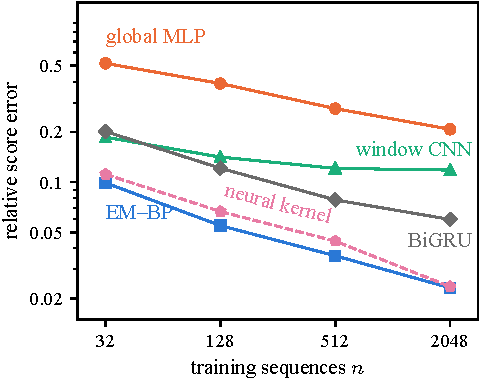
\includegraphics{fig_value_of_structure}
%% The plots and their style (box on all four sides, no grid, minor ticks, log scales, markers for measurements and
%% lines for closed forms) are made by tools/paper_figs/make_paper_figures.py in the research repository; see README.md.
%% The two diagrams are TikZ, \input from figures/*.tikz, so they use the body font and can be edited here.

%% ---------------------------------------------------------------- notation
\newcommand{\E}{\mathbb{E}}
\newcommand{\Normal}{\mathcal{N}}
\newcommand{\Kt}{K_\theta}
\newcommand{\dd}{\mathrm{d}}
\newcommand{\Dt}{\Delta_t}
\newcommand{\Ng}{N_g}

%% ---------------------------------------------------------------- writing aids
%% \note{...}    grey guidance text: what goes here, what Jerome asked for. Hide them all with \shownotesfalse.
%% \pending{...} a result that is not in yet (a run still on the cluster). Shown in orange so none is forgotten.
\newif\ifshownotes \shownotestrue
\definecolor{notegrey}{gray}{0.45}
\definecolor{pendingorange}{HTML}{C0501F}
\newcommand{\note}[1]{\ifshownotes{\color{notegrey}\itshape [#1]}\fi}
\newcommand{\pending}[1]{{\color{pendingorange}[pending: #1]}}

\graphicspath{{figures/draft-updated/}{figures/draft/}{figures/}}
\raggedbottom
\makeatletter
\setlength{\@fptop}{0pt}
\setlength{\@fpsep}{14pt plus 4pt}
\setlength{\@fpbot}{0pt plus 1fil}
\setlength{\@dblfptop}{0pt}
\setlength{\@dblfpsep}{14pt plus 4pt}
\setlength{\@dblfpbot}{0pt plus 1fil}
\makeatother
\usepackage{placeins}
\definecolor{jgbcolor}{RGB}{0,140,60}
\newcommand{\jgb}[1]{{\color{jgbcolor}#1}}
% draft-updated (20 Nov 2026): the one updated draft, with everything Jerome asked at the 18 Nov review (Overleaf notes,
% email of 17 Nov, pen notes at lunch): draft3's restructuring, draft4's runs, and the 20 Nov changes (DSM loss as the
% only metric, Figure 1 after his sketch, fewer formulas, L_DSM against phi2/phi1 in the main text, E80-E82, calcium).
% draft.tex (Jerome's) and main.tex are unchanged. The green box says what changed; \showreviewfalse hides it.
\newif\ifshowreview
\showreviewtrue
\newcommand{\review}[1]{\ifshowreview{\color{jgbcolor}#1}\fi}

\icmltitlerunning{Learning Scores for Markov Sequences in Generative Diffusion}

\begin{document}

\twocolumn[
\icmltitle{Learning Scores for Markov Sequences in Generative Diffusion}

\begin{icmlauthorlist}
  \icmlauthor{Giovanni Mantovani}{boc}
  \icmlauthor{J\'er\^ome Garnier-Brun}{boc}
  \icmlauthor{Marc M\'ezard}{boc}
\end{icmlauthorlist}
\icmlaffiliation{boc}{Department of Computing Sciences, Bocconi University, Milan, Italy}
\icmlcorrespondingauthor{Giovanni Mantovani}{giovanni-mantovani@studbocconi.it}
\icmlkeywords{diffusion models, belief propagation, expectation maximisation, Markov chains}
\vskip 0.3in
]

\printAffiliationsAndNotice{}

\begin{abstract}
Generative diffusion makes no assumption on the structure of the data it learns, which helps explain its reach but
leaves open when and how a denoiser exploits structure. We study one of the simplest structures, sequences generated by
a first-order Markov chain. It looks adversarial to diffusion: noise added independently to every entry makes the score
non-local. Yet the posterior of a clean sequence given its noisy version is still a chain, a tree, so belief propagation
(BP) gives the exact denoiser in $O(d)$ steps for a sequence of length $d$, for any transition kernel. We discretise
its messages on a grid, and learning the denoiser reduces to learning the transition kernel, a parametric family or a
small neural network, fitted by expectation--maximisation from noisy sequences or by maximum likelihood from clean
ones. We measure every model by the standard denoising score matching loss above its Bayes value. On a Laplace chain,
the neural kernel learned from noisy sequences has a 3 to 40 times smaller excess loss than a window CNN and 3 to 12
times smaller than a transformer and a bidirectional GRU trained on the clean sequences. On the stochastic Allen--Cahn
field, whose transition law changes shape with the state, the same comparison gives factors of 5 to 13 with 2{,}048
training sequences and 22 to 69 with 32{,}768.
% src: E89 (DSM rescoring of the frozen runs): Laplace per-seed median ratios over n = 32..2048, E56 energy (EM) vs E58
% window 3.3-37.5, vs E87 transformer 5.2-12.1, BiGRU 3.5-11.2 (all seeds win). Field, E55 energy_em, per-seed median
% ratios, 8/8 seeds win: n = 2048 window 12.8, transformer 5.4, BiGRU 5.2 (MLP 100); n = 32768 window 69.0,
% transformer 23.6, BiGRU 22.4 (MLP 464); E58 clean kernel vs window 211 at 2048 (with the E91 refits).
\end{abstract}

\ifshowreview
\noindent\fbox{\parbox{\dimexpr\columnwidth-2\fboxsep-2\fboxrule}{\scriptsize\color{jgbcolor}
\textbf{draft-updated (20 Nov): one draft with all of J\'er\^ome's 18 Nov review.} Hide with
\texttt{\textbackslash showreviewfalse}. Since draft4:
\begin{itemize}\setlength\itemsep{0pt}
\item Metric: the relative score error is retired. Every number and figure of the main text is the standard DSM loss
  (\cref{eq:dsm}) minus its Bayes value, computed exactly from the stored per-level errors of the frozen runs, or from
  the stored fitted kernels (\cref{app:measures}). Rankings are unchanged; ratios grow, the loss being a squared error.
\item Figure~1 redrawn after the sketch on the title page: noising, kernel and BP, one denoised chain, $L_{\rm DSM}$
  against $n$ with the Bayes loss.
\item Formulas: 8 displayed equations in the main text instead of 20; the Gaussian chain, the grid recursions and the
  kernel families are in the appendix.
\item $L_{\rm DSM}$ against $\phi_2/\phi_1$, EM against networks, in the main text (\cref{fig:nonmarkov}); new: BP plus
  a learned correction, which beats both BP and the BiGRU at every $\phi_2>0$.
\item New results: networks at their best (\cref{sec:results}), a tree with hidden nodes (\cref{sec:tree-hidden}).
\item New (21 Nov): do the generated samples copy the training sequences? No kernel ever does; networks trained to
  the end on 32 sequences do, none at their selected checkpoint (\cref{sec:memorization}, \cref{app:memorization-gen}).
\item New (21 Nov): the 29 clean-data fits of the neural kernel whose step size had collapsed are replaced by their
  refits, and EM at $n=32{,}768$ is in \cref{fig:results}a (\cref{app:em}).
\item Calcium imaging: synthetic and real (Spikefinder) runs submitted, \pending{results pending}.
\item Still in the relative score error (not yet converted, appendix only): \cref{tab:field}, \cref{fig:steps,fig:wall}.
\end{itemize}}}
\fi

\begin{figure*}[t]
  \centering
  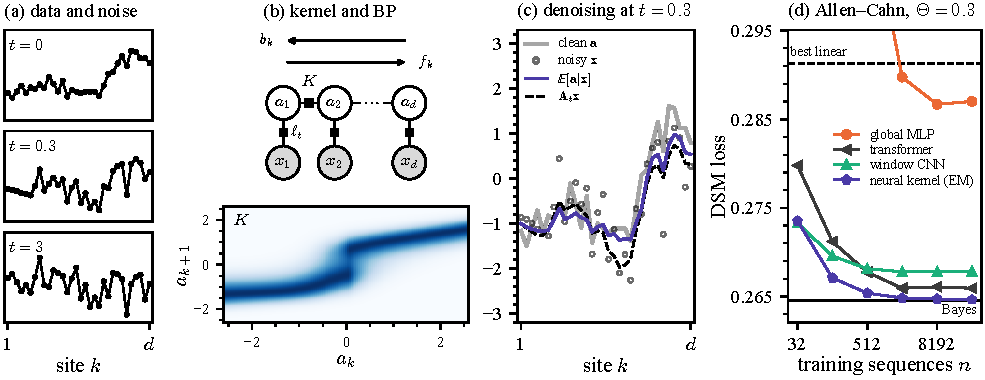
\includegraphics{fig_summary}
  \caption{Summary. (a) One sequence $\mathbf a$ of $d=32$ sites from the stochastic Allen--Cahn field, a first-order
  Markov chain, at three noise times: $\mathbf x_t=e^{-t}\mathbf a+\sqrt{\Delta_t}\,\boldsymbol\xi$ with
  $\Delta_t=1-e^{-2t}$ and $\boldsymbol\xi$ standard Gaussian (the same $\boldsymbol\xi$ at each $t$). (b) Top: the factor
  graph of the posterior of $\mathbf a$ given $\mathbf x$. Clean sites $a_k$ are white, noisy sites $x_k$ grey; black
  squares are the kernel factors $K(a_{k+1}\mid a_k)$ and the noise factors
  $\ell_t(x_k\mid a_k)=\mathcal N(x_k;e^{-t}a_k,\Delta_t)$. It is a chain, so belief propagation (BP), one forward sweep
  ($f_k$) and one backward sweep ($b_k$), is exact for any kernel $K$ and gives the posterior mean
  $\mathbb E[\mathbf a\mid\mathbf x]$, hence the score
  $\mathbf S_t(\mathbf x)=(e^{-t}\,\mathbb E[\mathbf a\mid\mathbf x]-\mathbf x)/\Delta_t$. Bottom: the neural kernel learned
  by expectation--maximisation (EM) from $n=2{,}048$ noisy sequences, as the density of $a_{k+1}$ given $a_k$ (each column
  scaled to its maximum): the next value jumps between the two wells of the field. (c) One sequence at $t=0.3$: the clean sequence $\mathbf a$, a sample of the stochastic Allen--Cahn field, which fluctuates by itself; the noisy sequence $\mathbf x$; the posterior mean $\mathbb E[\mathbf a\mid\mathbf x]$, computed by
  BP with the learned kernel; and $\mathbf A_t\mathbf x$, the best linear estimator of $\mathbf a$ from $\mathbf x$, with $\mathbf A_t=e^{-t}\boldsymbol\Sigma_0\boldsymbol\Sigma_t^{-1}$, $\boldsymbol\Sigma_t=e^{-2t}\boldsymbol\Sigma_0+\Delta_t\mathbf I$, where $\boldsymbol\Sigma_0$ is the covariance of the clean
  sequences. (d) Denoising score matching loss $L_{\rm DSM}$ on test sequences (mean over twelve noise levels $t\in[0.05,3]$) against the number $n$ of training sequences, medians over seeds. Solid line: the Bayes loss
  $L_{\rm Bayes}$, the loss of the exact score (computed by BP with the true kernel), which no denoiser can go below. Dashed: the best linear denoiser. The global MLP, the transformer and the window CNN are trained by denoising score
  matching; the neural kernel is learned by EM from noisy sequences and used inside BP. The global MLP is above the axis for $n\le512$.}
  \label{fig:summary}
  % src: tools/paper_figs/figs_v5.py::fig_summary_v5. (a) exact draw, Phi4Chain(T=0.3, h=1), seed 20261118, noise seed 7;
  % (b, c) E55 em_energy n = 2048 seed 0 (theta), grid and best linear from E58's context; (d) outputs/E89/dsm.csv.
\end{figure*}

\section{Introduction}
\label{sec:intro}

Diffusion models are state of the art when it comes to generating data with an a-priori unknown structure, from pictures
\cite{rombach2022latent,betker2023dalle3} and videos \cite{veo3} to protein structures \cite{abramson2024alphafold3};
see \cite{yang2023diffusion} for a review. Indeed, the reverse process transporting noise towards a desired data distribution
\cite{sohl2015deep,ho2020denoising,song2021scorebased} makes no prior assumption on the local or global nature of the
dependencies within data samples, notably explaining their performance in images, which carry correlations at all
scales without inherent directionality. While seemingly more adapted to next-token prediction due to its superficially
sequential aspect, text has increasingly also been found to be a modality where diffusion appears to be on par with, or
in some cases outperforms, next-token-prediction methods \cite{lou2024discrete,sahoo2024simple,nie2025large}.

The performance of generative diffusion and associated flow matching methods across such varied modalities remains
largely unexplained. While it now appears that the ability of networks to avoid memorizing training samples---despite
memorization being the optimum of the training loss \cite{gu2023memorization}---is largely related to some dynamical
regularization from gradient descent training, related to the simplicity bias observed across machine learning
\cite{bonnaire2025memorize,favero2025bigger}, when and how networks manage to generalize well is not clear
\cite{marion2026understanding}. As generalization must amount to extracting some underlying structure in data, much
effort is being dedicated to understanding how hidden structure, such as a latent tree model
\cite{sclocchi2025phase,garnierbrun2024transformers,mei2024unets}, as well as structure in the data support between
different modes \cite{biroli2023generative,biroli2024dynamical,achilli2026speciation,garnierbrun2026foam}, is learned by
architectures and revealed by the reverse process.

In this paper, we approach this question by considering data generated by a first-order Markov chain, a type of
structure that seems adversarial to generative diffusion. Indeed, as diffusion indiscriminately adds unstructured noise
to all entries in the sequence, it quickly leads a denoiser to be seemingly unable to exploit the locality of the
underlying data model (\cref{sec:gaussian}). Despite this, we show that an appropriately designed Markovian denoiser
structure can reach very good performance with a minimal model of the data. By exploiting the fact that the factor
graph of a Markov chain observed through noise is a tree (\cref{fig:summary}b), we write the denoiser as an exact belief
propagation (sum--product) message-passing algorithm running in $O(d)$ steps, with $d$ the dimension of the data. As we
consider data on a continuous support, the main obstacle is the distributional nature of the messages, which we overcome
with a simple discretization scheme. Learning to denoise is then reduced to learning the (possibly position-dependent)
transition kernel of the Markov chain. We propose both parametric forms for this kernel and a general neural
implementation. We finally show the efficiency of this denoising method on the stationary states of the stochastic
Allen--Cahn equation from statistical physics, where the neural kernel learned from noisy sequences outperforms standard
deep denoisers in the denoising loss, by a factor that grows with the data, and in data efficiency: from 512 sequences
its median loss is below that of every network trained on 32{,}768 (\cref{fig:summary}d). While we show that in
% src: E89 field excess, E55 energy_em n = 512 (median 8.1e-4) vs n = 32768: window, MLP, transformer 8/8 paired seeds,
% BiGRU 7/8 (median 1.16e-3).
this extreme case of a Markov chain, training on uncorrupted samples by maximum likelihood remains more effective than
learning from corrupted sequences, we believe that our factor-graph approach could be interesting where the Markov
structure is coupled to other latent models, to which it could perhaps be generalized.


\section{Setting}
\label{sec:setting}

\paragraph{Data model.}
We consider real-valued sequences $\mathbf{a}=(a_1,\ldots,a_d)\in\mathbb{R}^d$ generated by a first-order Markov chain,
\begin{equation}
p_0(\mathbf{a})=\mu(a_1)\prod_{k=1}^{d-1}K(a_{k+1}\mid a_k),
\label{eq:markov_prior}
\end{equation}
where $\mu$ is the law of the first site and $K(a'\mid a)$, a probability density in $a'$, is the transition kernel. We
assume a stationary chain with unit variance, so the same kernel acts at every position; with a kernel $K_k$ per
position every formula below holds with $K$ replaced by $K_k$.

\paragraph{Generative diffusion.}
Each coordinate is noised independently by the variance-preserving Ornstein--Uhlenbeck process
$dx_k=-x_k\,dt+\sqrt2\,dW_k$ \cite{song2021scorebased}, so that at time $t$, with $\Delta_t=1-e^{-2t}$,
\begin{equation}
x_k=e^{-t}a_k+\sqrt{\Delta_t}\,\xi_k,\qquad \xi_k\sim\mathcal{N}(0,1).
\label{eq:ou_corruption}
\end{equation}
The noise acts on each site separately, through the factor $\ell_t(x_k\mid a_k)=\mathcal{N}(x_k;e^{-t}a_k,\Delta_t)$,
so the posterior $p_t(\mathbf a\mid\mathbf x)$ is proportional to the prior \cref{eq:markov_prior} times
$\prod_k\ell_t(x_k\mid a_k)$. The score of the noisy data is the posterior mean, up to an affine map (Tweedie's formula
\cite{robbins1956empirical,efron2011tweedie}):
\begin{equation}
    \mathbf S_t(\mathbf x):=\nabla_{\mathbf x}\log p_t(\mathbf x)
    =\frac{e^{-t}\,\mathbb E[\mathbf a\mid\mathbf x]-\mathbf x}{\Delta_t}.
    \label{eq:tweedie}
\end{equation}

\paragraph{How we measure a denoiser.}
A score estimate $\widehat{\mathbf S}_t$ predicts the added noise as $\widehat{\boldsymbol\xi}=-\sqrt{\Delta_t}\,
\widehat{\mathbf S}_t(\mathbf x)$. Its denoising score matching (DSM) loss \cite{hyvarinen2005estimation,vincent2011connection,ho2020denoising},
\begin{equation}
    L_{\mathrm{DSM}}=\frac1d\,\mathbb E_{t,\mathbf a,\boldsymbol\xi}\big\|\boldsymbol\xi-\widehat{\boldsymbol\xi}\big\|^2,
    \label{eq:dsm}
\end{equation}
is the loss diffusion networks are trained on. We average it over twelve noise levels $t$ log-spaced between $0.05$
and $3$ and evaluate it on 2{,}048 test sequences. No denoiser does better than the exact posterior mean, so
$L_{\mathrm{DSM}}$ has a floor, the Bayes loss. On synthetic data we know the true kernel, and BP computes the exact
posterior mean (\cref{sec:tree}), so we report the excess $L_{\mathrm{DSM}}-L_{\mathrm{Bayes}}$, which is zero for
the exact score; on real data we report $L_{\mathrm{DSM}}$ itself.

\section{Exploiting Markov locality in the exact denoiser}
\label{sec:exact}

\subsection{The Gaussian chain}
\label{sec:gaussian}

The stationary Gaussian chain $a_{k+1}=\alpha a_k+\eta_k$, $\eta_k\sim\mathcal N(0,1-\alpha^2)$, is solvable in closed
form. Its precision matrix $\mathbf Q_0$ is tridiagonal, which is the algebraic form of the Markov property. The noisy
data stay Gaussian, and the score is linear, $\mathbf S_t(\mathbf x)=-\mathbf Q_t\mathbf x$, but $\mathbf Q_t$ is
dense for every $t>0$ (\cref{fig:locality}, \cref{app:gaussian-laplace}). Diffusion turns a locally structured chain
into a distribution whose score is not local. The effect is strongest at an intermediate noise level, $t^*\simeq0.075$
for $\alpha=0.85$, and fades at large $t$, where the noise dominates. So locality cannot simply be imposed on the
denoiser: one that only sees a window of neighbours cannot reach the exact score even with unlimited data. The
structure survives elsewhere: the posterior $p_t(\mathbf a\mid\mathbf x)$ is still a chain, because the noise adds one
factor per site and no new link.
% src: t* = 0.0753, fig_locality / fig_locality_curve

\subsection{Belief propagation on the noisy chain}
\label{sec:tree}

As a controlled non-Gaussian case we take the Laplace chain, $a_{k+1}=\alpha a_k+\varepsilon_k$ with Laplace noise of
variance $1-\alpha^2$: the same covariance as the Gaussian chain, but a sharp peak and heavier tails, and a score that
is no longer linear in $\mathbf x$. Its posterior is a chain with one extra factor per site (\cref{fig:summary}b,
\cref{fig:factor-graph}). It has no loop: it is a tree, where the cavity method and belief propagation are exact
\cite{mezard2001bethe,mezard2006reconstruction,mezard2009information}. The sum--product algorithm
\cite{pearl1988probabilistic,kschischang2001factor,yedidia2003understanding} computes the forward and backward messages
\begin{equation}
\begin{aligned}
    f_{k+1}(a')&=\ell_t(x_{k+1}\mid a')\textstyle\int K(a'\mid a)\,f_k(a)\,da,\\
    b_k(a)&=\textstyle\int K(a'\mid a)\,\ell_t(x_{k+1}\mid a')\,b_{k+1}(a')\,da',
\end{aligned}
\label{eq:bp}
\end{equation}
from $f_1=\mu\,\ell_t(x_1\mid\cdot)$ and $b_d=1$, and the posterior of site $k$ is proportional to $f_kb_k$; its mean
gives the score through \cref{eq:tweedie}. So, for any known first-order kernel, two sweeps give the exact joint score,
with no assumption of Gaussianity or linearity, in a number of steps linear in $d$. The noise level enters only through
$\ell_t$, so one kernel gives the score at every $t$. The same exact inference on a tree is at the heart of the
hierarchical models of \cite{garnierbrun2024transformers}, where transformers trained on such data learn to approximate
BP; a Markov chain is the simplest tree.

\subsection{Discretising the messages}
\label{sec:grid}

Each latent variable here is a real number, so a message is a density on $\mathbb R$, and the integrals of \cref{eq:bp}
have no closed form for a non-Gaussian kernel. We evaluate them on a uniform grid of $N_g=401$ points on $[-8,8]$: the
kernel becomes an $N_g\times N_g$ matrix, each integral a matrix--vector product, and a sequence costs $O(dN_g^2)$
operations (\cref{app:bp}). On the Gaussian chain, grid BP agrees with $-\mathbf Q_t\mathbf x$ to floating-point
rounding for every $t\geq0.05$, our smallest noise level, and on the Laplace chain 401 and 801 points give the same
DSM loss to $10^{-10}$ (\cref{fig:grid-vs-gaussian}). In the rest of the paper the exact score is grid BP with the true
kernel on 401 points.
% src: fig_grid_gaussian (exp_01/grid_sweep_M.csv); figs_v5._closure_dsm: grid 401 vs 801 excess median 4.3e-11 at t=0.05

\begin{figure}[t]
  \centering
  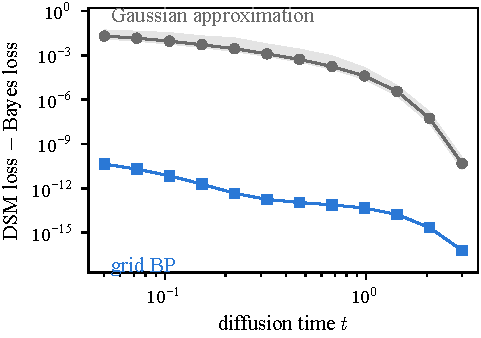
\includegraphics{fig_closure}
  \caption{What a Gaussian approximation costs on the Laplace chain ($\alpha=0.85$, $d=32$, true kernel): DSM loss
  above the Bayes loss at each noise level, for grid BP on the 401-point grid used in every experiment and for Gaussian
  messages, which give the best linear denoiser. Reference: grid BP on 801 points. Median over 2{,}000 sequences,
  10--90\% range shaded.}
  \label{fig:grid-vs-gaussian}
  % src: tools/paper_figs/figs_v5.py::fig_closure_dsm (reports/paper-figures/data/closure_dsm_2000.csv)
\end{figure}

Why not a Gaussian approximation, keeping only the mean and variance of each message? It is exact for the Gaussian
chain, but on the Laplace chain it gives back the score of the Gaussian chain with the same covariance, linear in
$\mathbf x$, which cannot see the peak of the Laplace law. This matters most at small noise, where the Laplace score is
close to a step (\cref{fig:laplace}). At $t=0.05$ its excess DSM loss is $2\times10^{-2}$, nine orders of magnitude
above grid BP (\cref{fig:grid-vs-gaussian}); the gap closes at large $t$, where both scores become that of isotropic
noise. This is also different from approximate message passing and Thouless--Anderson--Palmer methods
\cite{thouless1977solution,mezard1986sk,kabashima2003cdma,donoho2009message,krzakala2012statistical,bolthausen2014iterative},
built for dense systems where many weak interactions justify Gaussian messages with an Onsager correction
\cite{zdeborova2016statistical,mezard2017meanfield,lauditi2023sparse}. On a chain ordinary BP is already exact, so we
discretise the messages rather than approximate them.
% src: closure_dsm_2000.csv: t=0.05 lin_med 1.96e-2, grid_med 4.3e-11

\section{Learning the denoiser}
\label{sec:learning}

In practice the kernel is unknown and has to be learned from data. We work on the Laplace chain ($\alpha=0.85$,
$d=32$) and compare learning the kernel with training neural denoisers on the DSM loss.

\subsection{Expectation--maximisation through BP}
\label{sec:em}

Let $K_\theta$ be a family of kernels and $\mathbf{x}^{(1)},\ldots,\mathbf{x}^{(n)}$ noisy training sequences, each
observed at one noise level. The clean sequences are latent, and BP computes the likelihood of each noisy sequence from
the normalising constants of its forward messages. We maximise it by expectation--maximisation (EM)
\cite{dempster1977maximum}, as in the Baum--Welch algorithm for hidden Markov models \cite{baum1970,rabiner1989tutorial}:
the clean sequence is the hidden chain and the diffusion noise is the emission (\cref{fig:em-loop}). The E-step runs BP
with the current kernel and reads off the posterior of every pair of neighbouring sites,
$\xi_k(a,a')\propto f_k(a)K(a'\mid a)\ell_t(x_{k+1}\mid a')b_{k+1}(a')$; summed over sequences and links they give the
expected transition counts $\Xi(a,a')$. The M-step maximises
\begin{equation}
    Q(\theta)=\iint\Xi(a,a')\,\log K_\theta(a'\mid a)\,da\,da'.
    \label{eq:em-objective}
\end{equation}
With clean sequences $\Xi$ is the histogram of the observed transitions and the M-step is ordinary maximum likelihood;
with noisy ones the counts are soft, and BP provides them. Each M-step increases the likelihood
\cite{dempster1977maximum,wu1983}, BP enters only through $\Xi$, which stays fixed while $\theta$ moves, so nothing is
differentiated through the messages, and the noise level appears only in the E-step: the kernel is learned once and
gives the score at any noise level.

\subsection{Kernel families}
\label{sec:kernel-families}

We first use families with the shift form $a_{k+1}=\alpha a_k+\varepsilon_k$, where the noise $\varepsilon_k$ does not
depend on $a_k$: a mixture of $C=8$ Gaussians for the law of $\varepsilon_k$, with 25 parameters and an almost
closed-form M-step, and log-densities expanded in a Fourier series and three other bases, also with 25 parameters
(\cref{app:families}). They learn $\alpha$ quickly, but can only approximate the peak of the Laplace law. A kernel that
assumes nothing beyond the Markov property is the neural energy kernel, which we call the neural kernel:
\begin{equation}
    K_\theta(a'\mid a)=\frac{\exp[-E_\theta(a,a')]}{\int\exp[-E_\theta(a,u)]\,du},
    \label{eq:neural-kernel}
\end{equation}
with the normalisation computed on the grid and $E_\theta$ a network with two hidden layers of 16 units, 337 parameters.
It is a valid transition density for any weights. From noisy sequences it is learned by the same EM, the M-step taking
ten Adam steps \cite{kingma2015adam} on \cref{eq:em-objective}; from clean sequences, by maximising the likelihood
$\sum_{j,k}\log K_\theta(a^{(j)}_{k+1}\mid a^{(j)}_k)$ of the observed transitions, with no E-step at all.
\Cref{fig:families-main} shows what three of these kernels learn from noisy sequences.

\begin{figure}[t]
  \centering
  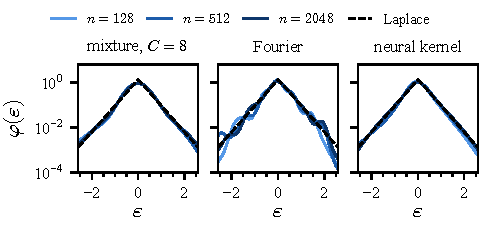
\includegraphics{fig_families_main}
  \caption{What three kernels learn by EM from $n=128$, $512$ and $2048$ noisy Laplace sequences: the learned kernel at
  the end of EM, as the law of $\varepsilon=a_{k+1}-\alpha a_k$ (for the neural kernel, $K_\theta(\varepsilon\mid
  a=0)$), against the Laplace law (dashed). One seed per $n$; all families in \cref{fig:families}.}
  \label{fig:families-main}
  % src: tools/paper_figs/figs_v3.py::fig_families_main (mixture thesis exp_18; E56 densities.csv seed 0)
\end{figure}

\subsection{Comparison with neural denoisers}
\label{sec:neural-denoisers}

Neural denoisers do not model the transition law: a network $\boldsymbol\epsilon_\phi(\mathbf x,t)$ predicts the noise
and is trained on the DSM loss \cref{eq:dsm} itself, with $\widehat{\boldsymbol\xi}=\boldsymbol\epsilon_\phi$. We use a
global MLP, which knows nothing about locality, a window CNN, which only looks at nearby sites, and two sequence models,
a transformer and a bidirectional GRU (26{,}016, 5{,}505, 18{,}057 and 15{,}169 parameters). All are trained on the
clean sequences with fresh noise at every step (\cref{fig:routes}), with hyperparameters chosen on separate seeds
(\cref{app:networks}, which also has a TCN and a U-Net).
% src: outputs/E03/winners.json, confirm.csv n_params (mlp 26,016; window 5,505)

\begin{figure*}[t]
  \centering
  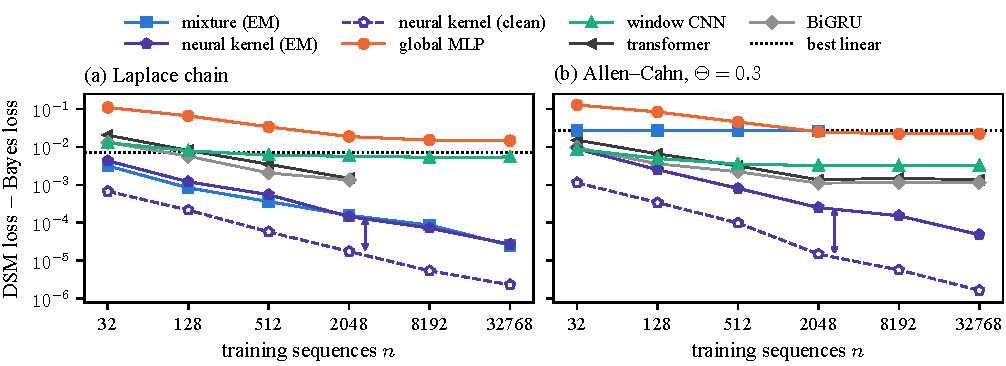
\includegraphics{fig_results}
  \caption{DSM loss above the Bayes loss against the number of training sequences $n$, medians over seeds. (a) Laplace
  chain, 16 seeds (8 for EM at $n\ge8192$ and for the transformer and BiGRU). (b) Allen--Cahn field at $\Theta=0.3$
  (\cref{sec:allen-cahn}), 8 seeds. Filled: kernels learned by EM from noisy sequences, used inside BP. Open, dashed: the
  neural kernel fitted on the clean sequences; arrow: the price of learning from noisy data. Networks: DSM on the clean
  sequences. Dotted: the best linear denoiser.}
  \label{fig:results}
  % src: tools/paper_figs/figs_v5.py::fig_results_dsm on outputs/E89/dsm.csv: (a) E02a+E86 mixture rescored from theta,
  % E56+E86 energy, E58 energy_h16/mlp/window/lmmse, E87 transformer/bigru; (b) E33 mixture rescored, E55 (per-level
  % relative errors x E58 field sq_ref), E58, E85. With the 29 E91 refits in place of the stalled E58 clean fits
  % (outputs/E91_dsm) and E86 at n=32768 (outputs/E86_dsm, E89's formula and checks): figs_v5.py::_dsm, 21 Nov 2026.
\end{figure*}

\paragraph{Results on the Laplace chain.}
\label{sec:results}
Each model is trained on $n$ sequences, from 32 to 2{,}048 with 16 seeds; EM was also run on 8{,}192 and 32{,}768 noisy sequences,
and with clean data $n$ goes up to 32{,}768. EM sees one noisy copy of each training sequence, at one of the twelve
levels; the networks see the clean sequences and draw fresh noise at every step. Every model keeps the checkpoint with
the lowest error on separate validation sequences, which matters for the networks, as they memorize small training
sets (\cref{sec:memorization}).

\Cref{fig:results}a shows the result. Both kernels learned by EM are below every network at every $n$. The neural kernel
learned from noisy sequences has an excess loss 3 to 40 times smaller than the window CNN and 25 to 130 times smaller
than the MLP, in every seed (median ratios from $n=32$ to 2{,}048). The CNN barely improves with more data and stays
near the best linear denoiser: this is the locality limit of \cref{sec:gaussian}. The transformer and the BiGRU keep
improving, but are still 12 and 11 times above the neural kernel at $n=2048$. The mixture, with 25 parameters,
is the best model up to $n=512$, 1.2 to 1.5 times below the neural kernel, which catches up at $n=2048$; EM on 8{,}192 and 32{,}768
noisy sequences improves both, though the mixture is still limited by its iteration budget there, and the neural
kernel at 8{,}192 (\cref{app:em}). Fitted on clean sequences, the neural kernel is another 5 to 9
times better---the gap between the open and filled markers (arrow) is the price of learning from noisy data---and from
128 clean sequences it is 25 times below the window CNN trained on 32{,}768.
% mixture vs neural kernel (E02a/E86 rescored vs E56/E86, per-seed median ratios nk/mix): 1.18, 1.54, 1.40, 0.96, 0.86.
% src: E89 dsm.csv, per-seed ratios (median, range): E56 energy vs E58 window 3.3 (n=32) ... 37.5 (2048), 16/16 every n;
% vs E58 mlp 24.5 ... 129.7, 16/16; vs E87 transformer 5.2 ... 12.1 (8/8), bigru 3.5 ... 11.2 (8/8); EM/clean (E56/E58
% energy_h16) 6.1, 5.0, 9.3, 8.7 (with the E91 refits; 8.1 before); clean n=128 2.16e-4 vs window n=32768 5.45e-3 (x25).

\paragraph{Networks at their best.} A large network should close the gap given enough data. We retrained the best
architectures with a learning-rate schedule and wider layers on up to $131{,}072$ clean sequences (\cref{app:networks}).
The best of them, a BiGRU, is three times better than with our standard recipe at $n=2048$, but still 3.5 times
above the neural kernel learned by EM from the same number of noisy sequences; it needs 16 times more sequences, all
clean, to reach it, and at $n=131{,}072$ it is still 4.5 times above the neural kernel fitted on 2{,}048 clean
sequences (same seeds). The kernels are
also much smaller (\cref{fig:params}).
% src: E80 (frozen 20 Nov 2026), E89 medians, seeds 0-3: bigru_h32 4.34e-4 at 2048 (E87 bigru 1.35e-3), bigru_h32
% 1.92e-4 at 8192, bigru_h128 1.19e-4 at 32768, 8.4e-5 at 131072; seeds 0-3: E56 energy EM at 2048 1.25e-4, E02a mixture
% 1.05e-4, E58 energy_h16 1.87e-5 (E91 refits; 1.91e-5 before), bigru_h128 at 131072 / clean = 4.50. read_e80 P1-P4, P6
% confirmed, P5 falsified (the window plateau was partly training).

\paragraph{Memorization.}
\label{sec:memorization}
With 32 training sequences, five of the six networks drive their training DSM loss far below the Bayes loss, $0.07$ to
$0.14$ against $0.27$, while their test loss rises to $0.5$--$0.75$: they memorize (\cref{app:memorization}); only the
window CNN does not. With 2{,}048 sequences training and test losses agree to within $0.01$. Their samples show it
too (\cref{app:memorization-gen}): trained to the end on 32 sequences, the global MLP reproduces a training sequence in
45 to 49\% of its samples and the BiGRU in 10 to 12\%, while no kernel, and no network at its selected checkpoint,
produces a copy at any $n$. BP with the clean-data neural kernel is 20 to 55 times closer to the Bayes loss than the
best network, at every $n$.
% src: read_e87 (E87): P1 5/6 networks (window not), P2 gaps at n=32 0.38-0.65 (window 0.04), at 2048 <= 0.0087; P4
% energy_clean below every network's best 8/8 at every n. Excess medians n=32: best net 1.30e-2 vs kernel 6.30e-4
% (x21); n=2048 1.35e-3 vs 2.45e-5 (x55)
% src: read_e92 (E92, frozen 21 Nov, outputs/hpc_E92_{laplace,field}): G1, G2 pass; P1, P2, P4 confirmed, P3 falsified
% (2 of 5 networks >= 0.1 at n=32 on the chain, needed 3), P5 falsified (kernel train-test gap up to 0.0043 > 2e-3,
% window CNN final gap on the field 0.036 < 0.05). frac_mem _final n=32 chain/field: mlp 0.448/0.492, bigru 0.103/0.122;
% every kernel and every _sel network 0 in every seed and n.

\subsection{Data that are not first-order Markov}
\label{sec:nonmarkov}

BP with a first-order kernel assumes first-order Markov data. To see what happens when this is wrong, we take
second-order chains, $a_k=\phi_1a_{k-1}+\phi_2a_{k-2}+\varepsilon_k$ with Laplace noise and $\phi_1$ adjusted so that
neighbouring sites keep correlation $0.85$; $\phi_2/\phi_1$ measures how much the second neighbour matters.

\begin{figure*}[t]
  \centering
  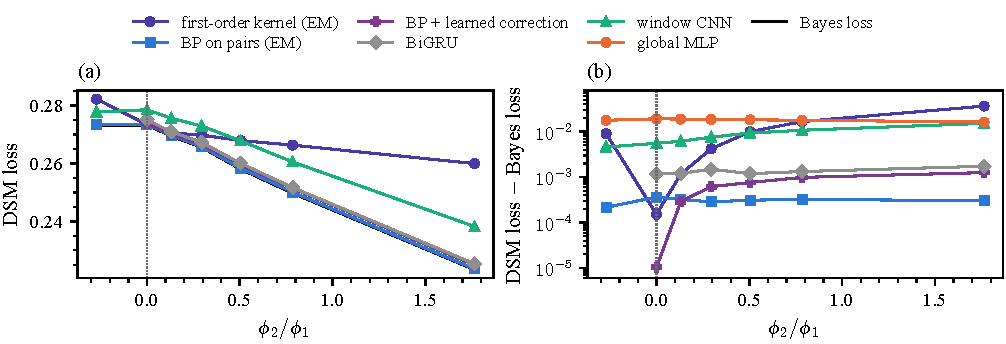
\includegraphics{fig_nonmarkov}
  \caption{Second-order chains against $\phi_2/\phi_1$, $n=2048$, medians over 8 seeds (4 for BP plus a learned
  correction and the BiGRU). (a) DSM loss; solid black: the Bayes loss. (b) DSM loss above the Bayes loss. At
  $\phi_2=0$ the data are first-order Markov.}
  \label{fig:nonmarkov}
  % src: tools/paper_figs/figs_v5.py::fig_nonmarkov_dsm on outputs/E89/dsm.csv (E62 first, pair, window, mlp; E81
  % hybrid_bigru, bigru, second-order families)
\end{figure*}

\Cref{fig:nonmarkov} shows what each model pays. The first-order kernel learned by EM is the best model at $\phi_2=0$
and stays below the window CNN up to $\phi_2=0.2$ ($\phi_2/\phi_1=0.3$) in every seed; beyond, its excess loss grows
with $\phi_2$ and follows that of the best possible first-order chain, so more data would not help: the model is wrong,
and from $\phi_2=0.3$ the CNN wins. The loss can be repaired in two ways. Pairs of neighbouring sites
$(a_{k-1},a_k)$ form a first-order chain again, so BP on pairs is exact, and EM on pairs stays between $2\times10^{-4}$
and $4\times10^{-4}$ at every $\phi_2$, below the best network in every seed, at the cost of one more grid dimension
per order. When the order is not known, BP with the first-order kernel can serve as the base of a network that learns
only a correction to its output: with the kernel and the network both trained on the clean sequences, this BP plus a
learned correction is below both BP and the BiGRU in every seed at every $\phi_2>0$, and equal to BP at $\phi_2=0$. Fractional Gaussian noise, the increments of fractional Brownian motion \cite{mandelbrot1968fractional},
is in \cref{app:nonmarkov}. There the kernel is learned as well as a first-order chain allows, within 7\% of the best one, but the window CNN wins already close to Markov: what decides
is the error of the best first-order chain, not the distance to it.
% src: E89 on E62 (n=2048, 8 seeds): first < window 8/8 at phi2 0, 0.1, 0.2; 1/8 at 0.3, 0/8 beyond; pair excess medians
% 2.2e-4..3.6e-4, pair < best net 8/8 every phi2. E81 (4 seeds): hybrid_bigru < both 4/4 at phi2 0.1..0.6; at phi2=0
% 1.04e-5 vs first 1.14e-5. E83 (DSM): first/floor1 1.014-1.068; window < first 8/8 at H = 0.3, 0.7, 0.8, 0.9, 5/8 at 0.6.

\section{Applications}
\label{sec:applications}

\subsection{The stochastic Allen--Cahn field}
\label{sec:allen-cahn}

The stochastic Allen--Cahn equation \cite{allen1979microscopic,dapratozabczyk2014} describes a field that relaxes in a
double-well potential $V(\phi)=\tfrac14(\phi^2-1)^2$ while being shaken by heat: it is the gradient flow
$\partial_\tau\phi=-\delta F/\delta\phi+\sqrt{2\Theta}\,\eta$ of the free energy
$F[\phi]=\int[\tfrac12(\partial_x\phi)^2+V(\phi)]\,dx$, with space-time white noise $\eta$ at temperature $\Theta$, and
its stationary law is $\exp(-F/\Theta)$. On a lattice of spacing $h$,
\begin{equation}
  p(\boldsymbol\phi)\propto\exp\Big(-\frac1\Theta\sum_i\Big[\frac{(\phi_{i+1}-\phi_i)^2}{2h}+hV(\phi_i)\Big]\Big),
  \label{eq:allen-cahn}
\end{equation}
a one-dimensional spin chain with continuous spins and nearest-neighbour couplings \cite{achilli2026speciation}, so
everything above applies. What makes it harder than the Laplace chain is that the \emph{shape} of the next value's law
depends on the current value: between the two wells it is broad, inside a well narrow and one-sided
(\cref{fig:summary}b, \cref{app:field}). We use $\Theta=0.3$, where the field sits in one well or the other with sharp
jumps between them (\cref{fig:summary}a), chains of $d=32$ sites and $h=1$, for which neighbouring sites have
correlation $0.85$, as on the Laplace chain.
% src: outputs/E32/cells.json (rho1 = 0.848 at T0.3_h1)

\Cref{fig:results}b compares the same models. The mixture assumes the shift form: its mean moves linearly with the
current value and its shape never changes, so its best member is close to a Gaussian chain, and it stays at the loss of
the best linear denoiser, from noisy and from clean data alike. The neural kernel has no such constraint and learns the
state-dependent law (\cref{fig:summary}b). From 2{,}048 noisy sequences its excess loss is 13 times below the window CNN,
100 times below the MLP and 5 times below the transformer and the BiGRU, in every seed; at $n=32{,}768$ the two sequence
models are still 22 to 24 times above it. Fitted on clean sequences, the neural kernel is 210 times below the CNN at
$n=2048$ and reaches the Bayes loss to within $2\times10^{-6}$ at $n=32{,}768$ (\cref{fig:summary}d).
% src: E89: E33 mixture rescored ~ E58 lmmse; E55 em_energy vs E58 window 12.8 (8/8), mlp 100 (8/8), E85 transformer
% 5.4, bigru 5.2 (8/8) at 2048; at 32768 23.6 and 22.4; E58 energy_h16 vs window 211 at 2048 (8/8; 189 before the E91
% refits); energy_h16 1.64e-6 at 32768 (1.74e-6 before).

\Cref{app:field} adds three higher temperatures and more kernels: every kernel whose shape can change with the current
value beats the best network trained on the same noisy data, and a kernel with the form of the lattice energy, with five
parameters, is the most accurate of all. A diffusion U-Net with $1.2\times10^{7}$ parameters, trained on the clean
sequences, needs four times more data than the neural kernel to reach the same error.
% src: figures/tab_field.tex; E55 finished cells (U-Net at n=8192 reaches the kernel's n=2048 error in every cell)

\subsection{Beyond chains: a tree with hidden nodes}
\label{sec:tree-hidden}

BP is exact on any tree, not only on chains. On a binary tree of depth five whose 32 leaves are the data and whose 31
internal nodes are never observed, with the Laplace kernel on every edge, EM through BP learns the kernel from noisy
leaves alone. From 2{,}048 sequences its excess loss is 33 to 46 times below the best of six networks (a BiGRU), and
assuming the wrong graph, a chain on the leaves, costs more than any network (\cref{app:tree}).
% src: E82 (frozen 20 Nov 2026) via E89: tree_energy 9.9e-5, tree_mixture 1.38e-4, bigru 4.54e-3, chain_mixture
% 2.30e-2 at n = 2048 (medians, 8 seeds); read_e82 P1-P5 confirmed.

\subsection{Calcium imaging}
\label{sec:calcium}

In two-photon calcium imaging \cite{vogelstein2009spike,friedrich2017fast,berens2018community}, the calcium
concentration in a neuron is a first-order chain that decays and jumps at each spike, and the recorded fluorescence is
this chain plus Gaussian noise: a fluorescence trace is the calcium chain already at a finite diffusion time. EM through
BP therefore learns the calcium kernel from fluorescence alone, and BP then gives the score of the diffused
fluorescence, its likelihood, and the posterior of the calcium, hence the spikes. \pending{Running: synthetic chains
with the exact score, and the ten Spikefinder datasets with simultaneous electrophysiology \cite{berens2018community}.}

\section{Conclusion}
\label{sec:conclusion}

For Markov sequences, the structure a denoiser can use is not in the score, which diffusion makes non-local, but in the
posterior, which stays a tree. BP turns a kernel, a function of two numbers, into the exact score at every noise level,
and EM learns the kernel from noisy data with BP as its E-step, without differentiating through it. A small neural
kernel removes the need to choose a parametric family and reaches a denoising loss one to three orders of magnitude
closer to the Bayes loss than networks with far more parameters. If the data are first-order Markov, it pays to learn
the kernel and let BP compute the score.

The method is not specific to diffusion. The same learned kernel gives, by BP, the posterior of a sequence observed with
Gaussian noise of any level, the likelihood of a noisy sequence, and new sequences by ancestral sampling; EM through grid
BP learns a nonparametric transition density of a hidden Markov chain from noisy observations alone, the setting of
state-space modelling, of which calcium imaging is one instance.

\paragraph{Limits.} The Markov order has to be known, or a network has to learn the correction; on pairs of sites a
grid step costs $O(N_g^3)$ instead of $O(N_g^2)$, and on data with long memory, such as fractional Gaussian noise, a
network can win even close to first-order Markov. Each site carries one number here; a state with $m$ numbers needs a
grid of $N_g^m$ points. The graph must be a tree, and the grid limits how small $t$ can be. Finally, a large network
closes the gap when clean data are plentiful, so the gain we measure is in data efficiency, which matters most where
scientific data are scarce.

\paragraph{Related work.} EM with forward--backward as the E-step is the classical way to fit hidden Markov and
state-space models \cite{baum1970,rabiner1989tutorial,shumway1982em,cappe2005}, and grids for non-Gaussian filtering go
back to \cite{kitagawa1987}; here the hidden chain is the clean data, the emission is the diffusion noise, and the
fitted model is used for its score. Diffusion models can also be trained from corrupted data
\cite{daras2023ambient,rozet2024learning,bai2024em}, but they learn a network score. Analytic and structured denoisers
\cite{kamb2024analytic,kadkhodaie2024generalization}, belief propagation on hierarchical data
\cite{garnierbrun2024transformers,sclocchi2025phase,mei2024unets} and the statistical physics of diffusion
\cite{biroli2023generative,biroli2024dynamical,achilli2025memorization,bonnaire2025memorize,garnierbrun2026biased,garnierbrun2026foam}
ask what structure a denoiser exploits. Markov sequences are the simplest, possibly non-Gaussian, case in which the
exact denoiser (up to discretization and kernel estimation error) is computable and can be learned from noisy data alone.

\section*{Impact statement}
This paper studies how much a denoiser for diffusion models can gain from knowing that its data are Markov, on
synthetic sequences, a simulated physical field and public calcium-imaging recordings with known ground truth. We see
no ethical concern specific to it.

\bibliography{references,references-updated}
\bibliographystyle{icml2026}

\newpage
\appendix
\onecolumn
\let\appendixsection\section
\renewcommand{\section}{\FloatBarrier\appendixsection}
\section{How the figures are measured}
\label{app:measures}

\paragraph{The DSM loss.} The test set has $m=2{,}048$ sequences of length $d=32$ at each of the twelve noise levels
$t\in\mathcal T$, log-spaced between $0.05$ and $3$, the same for every model. With $\widehat{\boldsymbol\xi}=
-\sqrt{\Delta_t}\widehat{\mathbf S}_t(\mathbf x)$, the noise $\boldsymbol\xi$ and the posterior mean of the noise
$\mathbb E[\boldsymbol\xi\mid\mathbf x]=-\sqrt{\Delta_t}\mathbf S_t(\mathbf x)$, the cross term in
$\|\boldsymbol\xi-\widehat{\boldsymbol\xi}\|^2$ has mean zero and $\mathbb E\,\xi_k^2=1$, so at each level
\begin{equation}
  \frac1d\,\mathbb E\|\boldsymbol\xi-\widehat{\boldsymbol\xi}\|^2
  =\underbrace{1-\frac{\Delta_t}{d}\,\mathbb E\|\mathbf S_t\|^2}_{\text{Bayes loss}}
  +\frac{\Delta_t}{d}\,\mathbb E\|\widehat{\mathbf S}_t-\mathbf S_t\|^2 .
  \label{eq:dsm-decomposition}
\end{equation}
We average both terms over the twelve levels. Every run stores, per level, the sums of $(\widehat S_{t,k}-S_{t,k})^2$
and of $S_{t,k}^2$ over the test set, with $\mathbf S$ from grid BP with the true kernel, so \cref{eq:dsm-decomposition}
gives the DSM loss, its Bayes value and the excess exactly, without new training. On the Laplace test set of seed 0 the
Bayes loss from \cref{eq:dsm-decomposition}, $0.2743$, agrees with the empirical loss of the true-kernel BP on one noise
draw, $0.2724$, to the sampling error of that draw. Runs that kept only an error pooled over levels (the mixture by EM)
were rescored from their stored kernels on their regenerated test sets, which reproduces their stored errors to
$2\times10^{-9}$;
the networks of \cref{app:memorization} were scored directly on the empirical DSM loss. The excess weights the levels by
$\Delta_t$, so, unlike a score error, it is not dominated by the smallest noise levels. The best linear denoiser,
dotted in the figures, is the linear function of $\mathbf x$ with the lowest DSM loss, computed from the exact covariance
of the chain.
% src: tools/core/e89_dsm_rescore.py (E89): outputs/E89/levels.csv, dsm.csv, rescored_checks.csv

\paragraph{Gaussian approximation against grid BP (\cref{fig:grid-vs-gaussian}).} We draw $2{,}000$ Laplace chains
($\alpha=0.85$, $d=32$) for each of the twelve levels and noise each one once. The reference is grid BP with the true
Laplace kernel on $801$ points, and we compare two estimates with it. The first is grid BP with the same kernel on the
$401$ points used in every experiment. The second is the Gaussian approximation: BP with Gaussian messages, which
replaces the Laplace noise by Gaussian noise of the same variance. Its posterior mean is that of the Gaussian chain with
the same covariance $(\boldsymbol\Sigma_0)_{ij}=\alpha^{|i-j|}$,
\begin{equation}
  \widehat{\mathbf m}=e^{-t}\boldsymbol\Sigma_0\big(e^{-2t}\boldsymbol\Sigma_0+\Delta_t\mathbf I\big)^{-1}\mathbf x,
\end{equation}
which is also the best linear denoiser. Each posterior mean goes into Tweedie's formula, and for each sequence we
compute the excess $\Delta_t\|\widehat{\mathbf S}_t(\mathbf x)-\mathbf S_t(\mathbf x)\|^2/32$ of
\cref{eq:dsm-decomposition}. The figure shows its median over the $2{,}000$ sequences at each level and its 10--90\%
range.
% src: tools/paper_figs/figs_v5.py::_closure_dsm (seed [20261108, round(1e4 t)]; reports/paper-figures/data/closure_dsm_2000.csv)

\paragraph{How far $\mathbf Q_t$ is from tridiagonal (\cref{fig:locality,fig:locality-curve}).} \Cref{fig:locality}
shows the magnitude $|(\mathbf Q_t)_{ij}|$ of every entry. To sum up a whole matrix in one number we use the Frobenius
norm of the entries at a given distance from the diagonal,
\begin{equation}
  \|\mathbf M\|_{|i-j|\ge2}=\Big(\sum_{|i-j|\ge2}M_{ij}^2\Big)^{1/2},
  \qquad
  \|\mathbf M\|_{|i-j|=1}=\Big(\sum_{|i-j|=1}M_{ij}^2\Big)^{1/2},
\end{equation}
and define
\begin{equation}
  r(t)=\frac{\|\mathbf Q_t\|_{|i-j|\ge2}}{\|\mathbf Q_0\|_{|i-j|=1}} .
\end{equation}
The numerator is the coupling between sites that are not neighbours, which is zero at $t=0$. The denominator is the
coupling between neighbours in the clean chain, a fixed scale. \Cref{fig:locality-curve} plots $r(t)$, and $t^{*}$,
the level framed in \cref{fig:locality}, is where $r$ is largest, found on a fine logarithmic grid of $t$.
% src: tools/paper_figs/make_paper_figures.py::_precision_snapshots (fig_ch05.dist_mass(Q_t, 2, L) / dist_mass(Q_0, 1, 1),
% 4,000 log-spaced t in [1e-3, 10^0.62]); t* = 0.0753

\paragraph{Parameter updates (\cref{fig:steps}).} The horizontal axis counts how many times the parameters change. For
the mixture, one update is one EM iteration: an E-step, which runs BP over all $n$ training sequences, and the
closed-form M-step. For the neural kernel, one update is one Adam step on $Q$ (\cref{eq:em-objective}); from noisy data
an EM iteration has one E-step and ten such steps, and from clean data there is no E-step. For a network, one update is
one Adam step on a batch of $64$ sequences. So the updates do not cost the same: an EM update uses every training
sequence and a network update uses $64$ of them. \Cref{app:compute} compares the methods in wall-clock time instead.
These two figures still show the relative score error
$\big(\sum\|\widehat{\mathbf S}-\mathbf S\|^2/\sum\|\mathbf S\|^2\big)^{1/2}$, pooled over levels, sequences and sites.
% src: tools/paper_figs/figs_v2.py::STEP_ARMS (energy scale x10); e63_curves_wall.csv

\section{The Gaussian and the Laplace chain}
\label{app:gaussian-laplace}

\begin{figure*}[!htbp]
  \centering
  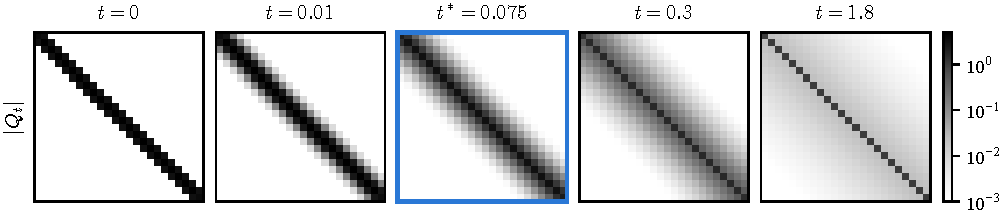
\includegraphics{fig_locality}
  \caption{Noise makes the score non-local. Magnitude of the matrix $\mathbf Q_t$ in the score
  $\mathbf S_t(\mathbf x)=-\mathbf Q_t\mathbf x$ of the Gaussian chain ($\alpha=0.85$, $d=24$) at five noise levels, on
  a log colour scale. At $t=0$ it is tridiagonal; at large $t$ it tends to the identity; in between, at
  $t^{*}\simeq0.075$ (framed), it is furthest from tridiagonal, as measured in \cref{app:measures}.}
  \label{fig:locality}
  % src: closed form, tools/paper_figs/make_paper_figures.py::fig_locality (t* = 0.0753 printed by the generator)
\end{figure*}

\paragraph{The Gaussian chain.} For $a_{k+1}=\alpha a_k+\eta_k$, $\eta_k\sim\mathcal N(0,1-\alpha^2)$, the clean
sequence is $\mathcal N(\mathbf 0,\boldsymbol\Sigma_0)$ with $(\boldsymbol\Sigma_0)_{ij}=\alpha^{|i-j|}$, and
$\mathbf Q_0=\boldsymbol\Sigma_0^{-1}$ is tridiagonal. Under \cref{eq:ou_corruption},
$p_t(\mathbf x)=\mathcal N(\mathbf 0,\boldsymbol\Sigma_t)$ with $\boldsymbol\Sigma_t=e^{-2t}\boldsymbol\Sigma_0+
\Delta_t\mathbf I$, and $\mathbf S_t(\mathbf x)=-\mathbf Q_t\mathbf x$ with $\mathbf Q_t=\boldsymbol\Sigma_t^{-1}$.

\paragraph{How non-local the Gaussian score gets.} \Cref{fig:locality-curve} follows the part of $\mathbf Q_t$ outside
the tridiagonal band as $t$ grows. It is zero at $t=0$, largest at $t^{*}\simeq0.075$, and it vanishes again at large
$t$, where $\mathbf Q_t$ tends to the identity. A denoiser that only sees a window of $r$ neighbours on each side cannot
reach the exact score even with unlimited data, and its best error falls only gradually as the window grows.

\begin{figure}[!htbp]
  \centering
  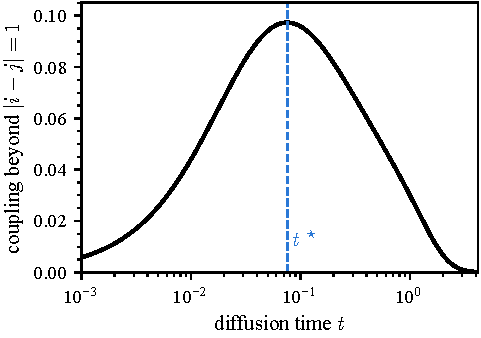
\includegraphics{fig_locality_curve}
  \caption{The ratio $r(t)$ of \cref{app:measures}: size of $\mathbf Q_t$ outside the tridiagonal band, relative to
  the nearest-neighbour entries of $\mathbf Q_0$, against $t$ (Gaussian chain, $\alpha=0.85$, $d=24$). It peaks at $t^{*}\simeq0.075$.}
  \label{fig:locality-curve}
\end{figure}

\paragraph{The Laplace chain against the Gaussian chain.} The two chains have the same covariance; only the law of the
noise $\varepsilon_k$ differs (\cref{fig:laplace}a). The Laplace law has a sharp peak at zero and exponential tails.
\Cref{fig:laplace}b--c show the score of the middle site of a chain of nine, as its own noisy value changes and the
others stay at zero. At small noise the Laplace score saturates. At large noise both scores are almost linear and almost equal. No linear denoiser can bend
like this, which is why the Gaussian approximation of \cref{fig:grid-vs-gaussian} fails at small noise.
% src: tools/paper_figs/thesis/fig_ch07.py grid_bp_score / gaussian_score (alpha=0.85, L=9, k=4), checked 8 Nov 2026

\begin{figure*}[!htbp]
  \centering
  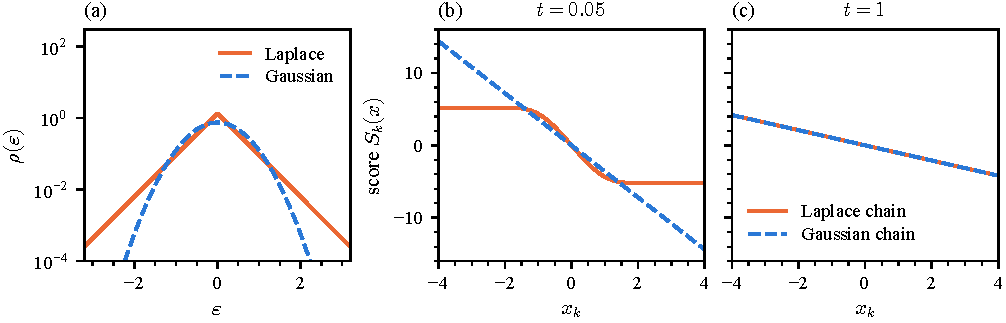
\includegraphics{fig_laplace}
  \caption{The Laplace chain. (a) Law of the noise $\varepsilon_k$, Laplace against Gaussian with the same variance.
  (b, c) Score of the middle site of a chain of nine against its own noisy value $x_k$, the other sites at zero, at
  $t=0.05$ and $t=1$. Exact scores from grid BP (Laplace) and in closed form (Gaussian).}
  \label{fig:laplace}
\end{figure*}

\section{Belief propagation on a grid}
\label{app:bp}

\begin{figure}[!htbp]
  \centering
  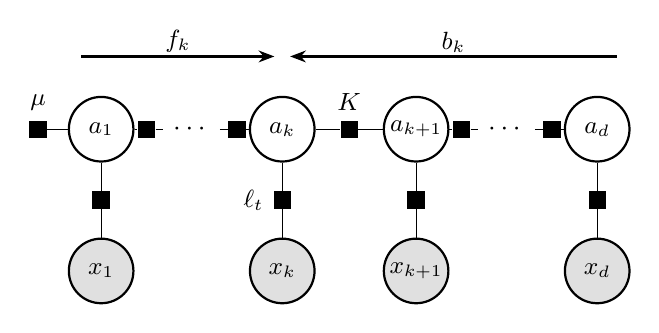
\begin{tikzpicture}[
    var/.style={circle,draw,thick,minimum size=8.2mm,inner sep=0pt,font=\small},
    obs/.style={circle,draw,thick,fill=black!12,minimum size=8.2mm,inner sep=0pt,font=\small},
    fac/.style={rectangle,fill=black,minimum size=2.2mm,inner sep=0pt},
    lab/.style={font=\small,inner sep=1pt},
    msg/.style={-{Stealth[length=2mm]},thick}]
  \node[var] (a1) at (0,0) {$a_1$};
  \node (d1) at (1.15,0) {$\cdots$};
  \node[var] (ak) at (2.3,0) {$a_k$};
  \node[var] (ak1) at (4.0,0) {$a_{k+1}$};
  \node (d2) at (5.15,0) {$\cdots$};
  \node[var] (ad) at (6.3,0) {$a_d$};
  \node[fac] (m0) at (-0.8,0) {};
  \draw (m0) -- (a1);
  \node[lab,above=0.8mm of m0] {$\mu$};
  \foreach \u/\v/\n in {a1/d1/ka,d1/ak/kb,ak/ak1/kc,ak1/d2/kd,d2/ad/ke} {
    \node[fac] (\n) at ($(\u)!0.5!(\v)$) {};
    \draw (\u) -- (\n) -- (\v);
  }
  \node[lab,above=0.8mm of kc] {$K$};
  \foreach \i/\n in {a1/1,ak/k,ak1/{k+1},ad/d} {
    \node[fac] (o\i) at ($(\i)+(0,-0.9)$) {};
    \node[obs] (x\i) at ($(\i)+(0,-1.8)$) {$x_{\n}$};
    \draw (\i) -- (o\i) -- (x\i);
  }
  \node[lab,left=0.8mm of oak] {$\ell_t$};
  \draw[msg] ($(a1.north)+(-0.25,0.5)$) -- node[lab,above]{$f_k$} ($(ak.north)+(-0.1,0.5)$);
  \draw[msg] ($(ad.north)+(0.25,0.5)$) -- node[lab,above]{$b_k$} ($(ak.north)+(0.1,0.5)$);
\end{tikzpicture}

  \caption{Factor graph of the posterior $p_t(\mathbf a\mid\mathbf x)$. White circles are the clean values $a_k$, grey
  circles the noisy observations $x_k$, which are known. Black squares are the factors: the law $\mu$ of the first site,
  the kernel $K(a_{k+1}\mid a_k)$ between neighbours and the noise term $\ell_t(x_k\mid a_k)$ at each site. There is no
  loop, so belief propagation is exact. The forward message $f_k$ carries what $x_1,\ldots,x_k$ say about $a_k$, the
  backward message $b_k$ what $x_{k+1},\ldots,x_d$ say about it, and the posterior of $a_k$ is proportional to
  $f_k(a_k)\,b_k(a_k)$.}
  \label{fig:factor-graph}
\end{figure}

\paragraph{Recursions.} The grid is $g_i=-A+ih$, $i=0,\ldots,N_g-1$, $h=2A/(N_g-1)$, with $A=8$, $N_g=401$
($h=0.04$) and trapezoidal weights $w_i$; the kernel is the matrix $K_{ij}=K(g_i\mid g_j)$ and the noise term the vector
$(\ell_k)_i=\ell_t(x_k\mid g_i)$. Each column of the kernel matrix is normalised so that
$\sum_iw_iK_{ij}=1$, and $\mu$ is the law of the first site on the grid. The forward sweep is
\begin{equation}
  \tilde f_1=\mu\odot\ell_1,\qquad
  \tilde f_k=\ell_k\odot K\,(w\odot f_{k-1}),\qquad
  c_k=\sum_iw_i\tilde f_k(i),\qquad f_k=\tilde f_k/c_k ,
\end{equation}
and the backward sweep is
\begin{equation}
  b_d=\mathbf 1,\qquad
  \tilde b_k=K^{\top}\big(w\odot\ell_{k+1}\odot b_{k+1}\big),\qquad
  b_k=\tilde b_k\big/\textstyle\sum_iw_i\tilde b_k(i).
\end{equation}
The normalisations keep the numbers in floating-point range and do not change the result. The posterior mean of site
$k$ is the weighted average of the grid points with weights $w\odot f_k\odot b_k$. The pair posterior used by the E-step
is
\begin{equation}
  \xi_k(i,j)\propto f_k(j)\,w_j\,K_{ij}\,w_i\,\ell_{k+1}(i)\,b_{k+1}(i)
  \approx\Pr(a_k=g_j,\,a_{k+1}=g_i\mid\mathbf x),
\end{equation}
normalised to sum to one, and the log-likelihood of a sequence is $\log p(\mathbf x)=\sum_k\log c_k$, which comes from the forward sweep.

\paragraph{Accuracy.} The grid spacing must resolve the noise term, whose width in $a$ is about $\sqrt{2t}$ at small $t$:
at $t=0.05$ it is $0.32$, eight times the spacing $h=0.04$. With $A=8$ the probability that falls outside the grid is
negligible. On the Gaussian chain, where the exact score is $-\mathbf Q_t\mathbf x$, grid BP reaches double-precision
round-off for $t\geq0.05$ already with 101 points (\cref{fig:grid}). On the Laplace chain we compare 401 with 801
points: over 2{,}000 sequences the DSM loss differs by $4\times10^{-11}$ at $t=0.05$, and by less at larger $t$
(\cref{fig:grid-vs-gaussian}).
% src: figs_v5._grid_gauss_dsm (excess ~1e-30 for t >= 0.05 at 101, 201, 401 points; 101 points: 1e-5 at t = 0.005);
% figs_v5._closure_dsm (closure_dsm_2000.csv)

\begin{figure}[!htbp]
  \centering
  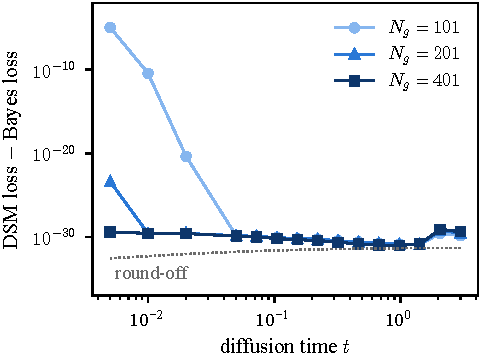
\includegraphics{fig_grid_gaussian}
  \caption{Grid BP against the exact score $-\mathbf Q_t\mathbf x$ of the Gaussian chain ($\alpha=0.85$, $d=32$) for
  three grid sizes: DSM loss above the Bayes loss, median over 2{,}000 sequences. Dotted: the excess that a relative
  error of double-precision round-off on the score would give.}
  \label{fig:grid}
  % src: tools/paper_figs/figs_v5.py::fig_grid_gaussian_dsm (reports/paper-figures/data/grid_gauss_dsm_2000.csv)
\end{figure}

\section{Learning details}
\label{app:em}

\begin{figure}[!htbp]
  \centering
  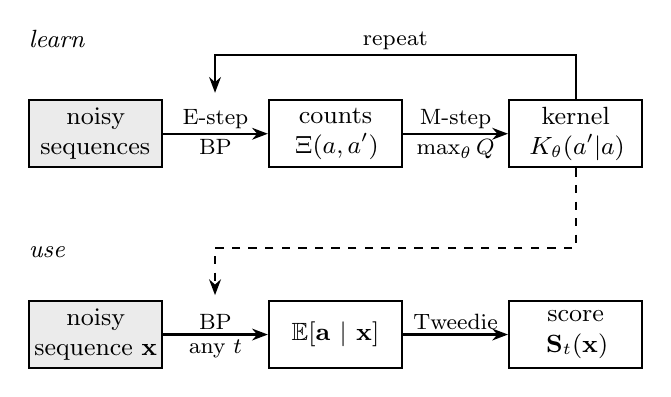
\begin{tikzpicture}[
    box/.style={draw,thick,align=center,font=\small,minimum height=8.5mm,inner sep=2pt,text width=1.55cm},
    data/.style={box,fill=black!8},
    arr/.style={-{Stealth[length=2mm]},thick},
    lab/.style={font=\footnotesize,align=center,inner sep=1.5pt},
    stage/.style={font=\small\itshape,anchor=west,inner sep=0pt}]
  \node[stage] at (-0.85,1.2) {learn};
  \node[data] (x) at (0,0) {noisy\\ sequences};
  \node[box] (xi) at (3.05,0) {counts\\ $\Xi(a,a')$};
  \node[box] (k) at (6.1,0) {kernel\\ $K_\theta(a'|a)$};
  \draw[arr] (x) -- node[lab,above]{E-step} node[lab,below]{BP} (xi);
  \draw[arr] (xi) -- node[lab,above]{M-step} node[lab,below]{$\max_\theta Q$} (k);
  \draw[arr] (k.north) |- node[lab,above,pos=0.75]{repeat} (1.52,1.0) -- (1.52,0.52);
  \node[stage] at (-0.85,-1.5) {use};
  \node[data] (y) at (0,-2.55) {noisy\\ sequence $\mathbf{x}$};
  \node[box] (m) at (3.05,-2.55) {$\mathbb{E}[\mathbf{a}\mid\mathbf{x}]$};
  \node[box] (s) at (6.1,-2.55) {score\\ $\mathbf{S}_t(\mathbf{x})$};
  \draw[arr] (y) -- node[lab,above]{BP} node[lab,below]{any $t$} (m);
  \draw[arr] (m) -- node[lab,above]{Tweedie} (s);
  \draw[thick,dashed,-{Stealth[length=2mm]}] (k.south) |- (1.52,-1.45) -- (1.52,-2.05);
\end{tikzpicture}

  \caption{Learning and using the kernel. Learn: BP with the current kernel gives the posterior of every pair of
  neighbouring sites, summed into the expected transition counts $\Xi$ (E-step); the kernel is refitted to these
  counts (M-step); repeat. Use: BP with the learned kernel gives $\mathbb E[\mathbf a\mid\mathbf x]$, and so the score,
  at any noise level. BP enters the learning only through $\Xi$, so nothing is differentiated through BP.}
  \label{fig:em-loop}
\end{figure}

\paragraph{Data and selection.} Each clean training sequence is noised once, at one of the twelve noise levels, so EM
sees $n$ noisy sequences in all. The networks instead see the clean sequences and draw fresh noise at every step. EM runs
up to 1{,}200 iterations (2{,}400 for the neural kernel) and keeps the kernel at fixed checkpoints; every model, kernel or
network, is tested at the checkpoint with the lowest score error on 1{,}024 validation sequences. Without the exact
score, EM can select by the likelihood of noisy validation sequences, which BP computes, and a network by its validation
loss.
% src: experiments/e03_baselines.py::_one_view_groups; outputs/E02a/params_capacity.json; tools/core/read_e65.py (E65):
% free/oracle max em_bp 1.7%, spline 6.9%, energy 6.9%, networks <= 3.4%

\paragraph{Training-set sizes.} On the Laplace chain, EM from noisy sequences was run for $n$ from 32 to 2{,}048 with
16 seeds and at $n=8{,}192$ and $32{,}768$ with 8 seeds, while the clean-data kernel and the networks go up
to 32{,}768. The larger sizes were added later, to ask whether the
networks catch up with the kernel given much more data. From clean data
the transition counts $\Xi$ are computed once, in a few milliseconds, and an M-step then costs the same at every $n$.
From noisy data every EM iteration runs BP over all $n$ sequences, so its cost grows in proportion to $n$: $3.4$\,s at
$n=2{,}048$ for the mixture (\cref{app:compute}), about a minute at $n=32{,}768$, which makes 15 to 30 hours per fit and
seed over the 1{,}200 to 2{,}400 iterations. At $n=8{,}192$ EM had the same iteration budget as at $n=2{,}048$, and it
was not enough: the mixture was still improving on the validation sequences at its last checkpoint (1{,}200 iterations)
in 7 of 8 seeds, and the neural kernel ran out of its 2{,}400 iterations in 4 of 8. The $n=8{,}192$ points of
\cref{fig:results}a are therefore what EM reaches with that budget, not with that much data. At $n=32{,}768$ the mixture
was again still improving at its last checkpoint, in all 8 seeds, while the neural kernel met its stopping rule in every
seed, after 786 to 2{,}377 iterations. Paired by seed, the mixture at $n=8{,}192$ is below its own loss at $n=2{,}048$ in
5 of 8 seeds and the neural kernel in 6 of 8, and at $n=32{,}768$ both are below their loss at $n=8{,}192$, in 7 and 8
of 8 seeds; at $n=32{,}768$ the two kernels are level (median ratio 0.94). The price of noisy data, the ratio of the EM
neural kernel to the clean-data one, is 9 at $n=2{,}048$, 16 at $n=8{,}192$ and 10 at $n=32{,}768$ (medians of the
per-seed ratios). A rerun at $n=8{,}192$ with four times the iteration budget is \pending{running}.
% src: E86 (frozen 19 Nov 2026, outputs/hpc_E86_n8192): capacity.csv at_cap 7/8 with val_curve still falling at 1200;
% kernels.csv stop_reason censored 4/8 (n_iters 2401); read_e86 P1 8192<2048 5/8; medians energy 0.0171, energy_h16
% 0.0045 (seed mean ratio 0.95 because E58's clean fit at n=8192 seed 1 stalled at 0.1228: registered P2 FALSIFIED as
% worded). n=32768 (frozen 21 Nov, outputs/hpc_E86_n32768; DSM by tools/core/e86_dsm.py, C2 8.0e-10): read_e86 P1
% FALSIFIED (8192<2048 5/8, 32768<8192 7/8), P2 FALSIFIED as worded on the original E58 rows (8192 0.95, 32768 3.62),
% P3 CONFIRMED. DSM with the E91 refits: mixture 32768<8192 7/8, energy 8/8; mixture at_cap 8/8 (checkpoint 1200);
% energy stop_reason converged 8/8 (786-2377 iters); medians 32768 mix 2.53e-5, energy 2.71e-5, nk/mix 0.94 (mix<nk
% 3/8); EM/clean median per-seed ratio 8.7 / 15.8 / 10.4 at 2048 / 8192 / 32768.
% src: E58 registry (sizes 32..32768 added 31 Oct for the clean arms; clean Xi 5 ms at N = 2048; M-step does not depend
% on N); E63 timing 3.4 s / 2.5 s per EM iteration at N = 2048 -> x16 = 54 s / 40 s; x1200 / x2400 = 18 h / 27 h

\paragraph{M-steps.} For the mixture, the M-step is a closed-form update \cite{meng1993maximum}: each component's weight,
mean and variance are the weighted frequency, mean and variance of the residuals $g_i-\alpha g_j$, with weights $\Xi_{ij}$
times the component's responsibility, and $\alpha$ is then a weighted least-squares slope. For the Fourier kernel and
the other log-linear families, $Q$ is concave and its gradient is the observed minus the expected value of each basis
function, so a few gradient steps per iteration are enough. For the neural kernel, each M-step takes ten Adam steps on
$Q$, differentiating only through the network and its normalisation on the grid, and halves the step size whenever $Q$
does not increase.

\paragraph{Clean-data fits.} From clean sequences the neural kernel is fitted by the same Adam steps and the same step
halving, on the likelihood itself. In 29 of its 144 clean fits on the two data sets of \cref{fig:results}, the halving
drove the step size below $10^{-6}$, which freezes the fit; five of them had stopped near the loss of the best linear
denoiser. We refitted these 29 from the same initialisation, with the same data and budget, restarting Adam after every
rejected step, and report the refits. None of them stalls again, and they lower the medians of \cref{fig:results} by at
most 23\%.
% src: E91 (registered 20 Nov 2026; stalled list outputs/E91_list/stalled.csv written before submission; frozen
% outputs/hpc_E91_r0 21 Nov): read_e91 G1 pass, P1-P3 confirmed, no restart needed. DSM: tools/core/e91_dsm.py (same
% bundles: sq_ref equal to E58's, C2 4e-14). Truly stuck: laplace s1, s8 at 8192; field s2 at 8192, s6, s7 at 512.
% Median changes: laplace 8192 -23.3%, 32768 -15.2%; field 512 -19.9%, 2048 -8.7%, 8192 -4.3%, 32768 -5.9%; others 0.

\section{Training time}
\label{app:compute}

On one CPU thread at $n=2048$, an EM iteration takes $3.4$\,s for the mixture and $2.5$\,s for the neural kernel,
because BP runs over every training sequence; a clean-data iteration of the neural kernel takes $0.5$\,s. An SGD step
takes $2.5$\,ms for the window CNN and $1.0$\,ms for the MLP. \Cref{fig:steps} counts parameter updates: the mixture passes the final error of the window CNN after 20 EM
iterations and is close to its own best after about 160; the neural kernel passes it after 400 Adam steps from noisy
data and 200 from clean data; the CNN needs all of its 32{,}000 steps, and the transformer and the BiGRU are still
improving at 32{,}000 steps. \Cref{fig:wall} redraws it against time.
From clean data the neural kernel reaches the final error of each network before the network does, in every seed. From
noisy data the networks are cheap per step and stop improving early, so they reach their own final error first, at five
to nine times the error of the kernels. At test time, BP on the 401-point grid takes about $7$\,ms per sequence for all
twelve noise levels. However, reducing the number of points on the grid notably reduces the time consumed.
% src: outputs/hpc_E63/timing.csv (E63, tools/core/read_e63.py D1); e63_curves_wall.csv at N = 2048

\begin{figure}[!htbp]
  \centering
  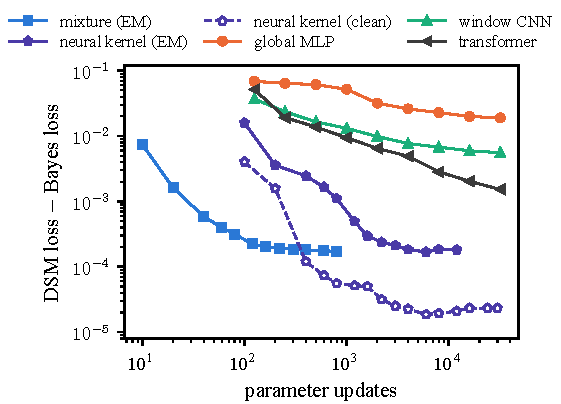
\includegraphics{fig_steps}
  \caption{Step efficiency on the Laplace chain with $n=2048$: relative score error on the test sequences against the
  number of parameter updates. One update is an EM iteration of the mixture, one Adam step of the neural kernel (ten per EM iteration), or
  one Adam step of a network on 64 sequences (\cref{app:measures}). Median over 16 seeds; transformer and BiGRU:
  retrained with the same data and recipe, 8 seeds.}
  \label{fig:steps}
  % src: tools/paper_figs/figs_v4.py::fig_steps_v4: figs_v2's curves (reports/core/e63_curves_wall.csv, E65 refits,
  % frozen 4 Nov 2026) + E87 curves.csv test_risk at n = 2048 (transformer, bigru)
\end{figure}

\begin{figure}[!htbp]
  \centering
  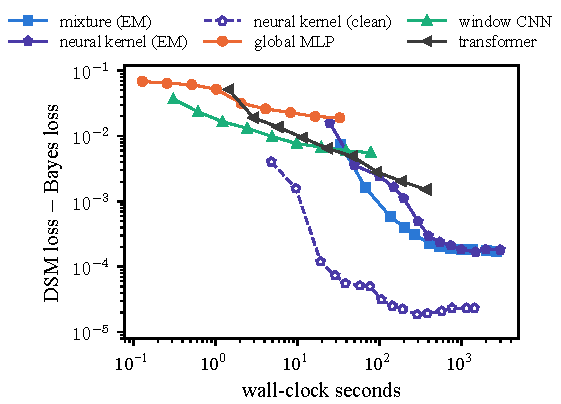
\includegraphics{fig_wall}
  \caption{The curves of \cref{fig:steps} against wall-clock seconds on one CPU thread ($n=2048$, median over 16
  seeds; without the transformer and the BiGRU, which were not timed per step).}
  \label{fig:wall}
  % src: tools/paper_figs/figs_v2.py::fig_wall on reports/core/e63_curves_wall.csv
\end{figure}

\section{Other kernel families}
\label{app:families}

\paragraph{Shift families.} The mixture writes the kernel as
$K_\theta(a'\mid a)=\sum_{c=1}^{8}\pi_c\,\mathcal N(a'-\alpha a;\nu_c,s_c^2)$, with weights summing to one: 25 parameters.
It learns $\alpha$ to $0.1\%$ from 512 sequences. Four other families write the log-density of the noise as
\begin{equation}
  \log\varphi_\theta(\varepsilon)=-\frac{\lambda\varepsilon^2}{2}+\sum_{m=1}^{23}c_m\,b_m(\varepsilon)-\log Z_\theta,
\end{equation}
with the basis evaluated on $[-4,4]$ and held constant beyond it, where the quadratic term with learned $\lambda>0$ takes
over. With $\alpha$ and $\lambda$ each family has 25 parameters, like the mixture. The bases are cubic B-splines with
equally spaced knots, Gaussian bumps with equally spaced centres, a Fourier series ($\cos(m\pi\varepsilon/4)$ for
$m\le12$ and $\sin(m\pi\varepsilon/4)$ for $m\le11$) and Legendre polynomials. Splines and bumps are local and can
bend sharply at one point, as the Laplace peak requires; Fourier and Legendre are global and can only approximate it by
oscillating.

\paragraph{A kernel without the shift form.} The log-linear kernel writes $\log K_\theta(a'\mid a)$ in a $10\times10$
basis of B-splines in both arguments, 100 parameters, and is learned like the other log-linear families.

\paragraph{Results.} \Cref{fig:families} shows what each family learns, and \cref{fig:families-error} its error. The
four bases behave like the mixture: Fourier and Legendre oscillate in the tails, but the tails carry little
probability, and their excess DSM losses are 0.8 to 1.6 times that of the mixture. All five shift families are
below the best of six networks at every $n$. The log-linear kernel learns slowly, because its 100 parameters are spread
over the whole plane, and it is the only kernel that loses to a network, the window CNN. The neural kernel is the
closest to the true kernel of all the families.
% src: E89 medians, family/mixture at n = 32..2048: fourier 1.00-1.63, spline 0.85-1.32, rbf 0.92-1.29, legendre
% 0.84-1.50. tools/core/read_e56.py (E56): P4 loglinear2d vs window 0/16, P5 Hellinger
% energy 0.0394 (smallest), shift bases 0.046-0.049, loglinear2d 0.1071

\begin{figure*}[!htbp]
  \centering
  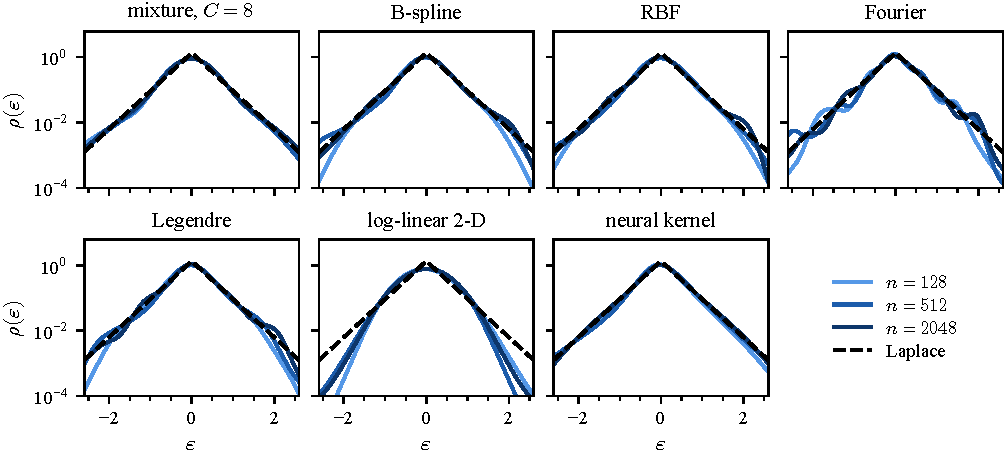
\includegraphics{fig_families}
  \caption{What each kernel family learns from noisy sequences, from $n=128$, $512$ and $2048$ sequences, against the
  Laplace law (dashed). Each curve is the learned kernel itself at the end of EM, evaluated on the grid: for the shift
  families the law $\varphi_\theta$ of the noise $\varepsilon=a_{k+1}-\alpha a_k$, and for the two families without the
  shift form the learned $K_\theta(\varepsilon\mid a=0)$. One seed per $n$.}
  \label{fig:families}
  % src: mixture thesis exp_18 (density file); the six others outputs/hpc_E56_s*/densities.csv, seed 0
\end{figure*}

\begin{figure}[!htbp]
  \centering
  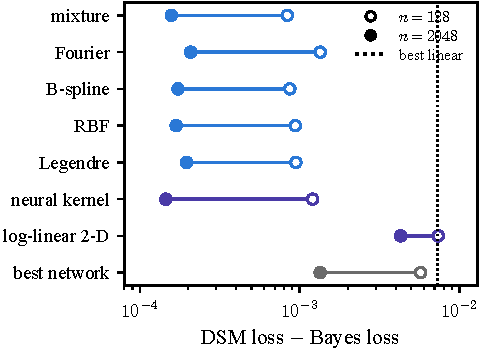
\includegraphics{fig_families_error}
  \caption{DSM loss above the Bayes loss of every kernel family learned by EM, and of the best of the six networks,
  from $n=128$ (open) and $n=2048$ (filled) sequences. Blue: families with the shift form; purple: families without it.
  Dotted: the best linear denoiser. Laplace chain, medians over seeds (16 for the kernels, 8 for the networks), same
  test sequences.}
  \label{fig:families-error}
  % src: tools/paper_figs/figs_v5.py::fig_families_error_dsm (E89: E02a mixture rescored, E56, E87 networks, E58 lmmse)
\end{figure}

\section{Other networks}
\label{app:networks}

\begin{figure}[!htbp]
  \centering
  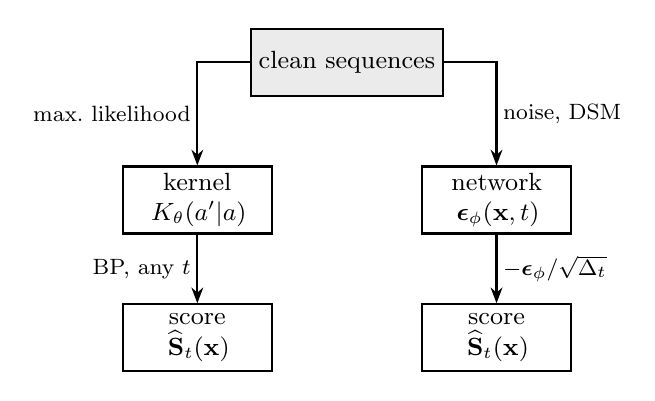
\begin{tikzpicture}[
    box/.style={draw,thick,align=center,font=\small,minimum height=8.5mm,inner sep=2pt,text width=1.75cm},
    data/.style={box,fill=black!8,text width=2.3cm},
    arr/.style={-{Stealth[length=2mm]},thick},
    lab/.style={font=\footnotesize,align=center,inner sep=2pt}]
  \node[data] (a) at (0,0) {clean sequences};
  \node[box] (k) at (-1.9,-1.75) {kernel\\ $K_\theta(a'|a)$};
  \node[box] (n) at (1.9,-1.75) {network\\ $\boldsymbol{\epsilon}_\phi(\mathbf{x},t)$};
  \node[box] (s1) at (-1.9,-3.5) {score\\ $\widehat{\mathbf{S}}_t(\mathbf{x})$};
  \node[box] (s2) at (1.9,-3.5) {score\\ $\widehat{\mathbf{S}}_t(\mathbf{x})$};
  \draw[arr] (a.west) -| node[lab,left,pos=0.75]{max.\ likelihood} (k.north);
  \draw[arr] (a.east) -| node[lab,right,pos=0.75]{noise, DSM} (n.north);
  \draw[arr] (k) -- node[lab,left]{BP, any $t$} (s1);
  \draw[arr] (n) -- node[lab,right]{$-\boldsymbol{\epsilon}_\phi/\sqrt{\Delta_t}$} (s2);
\end{tikzpicture}

  \caption{Two ways to learn from the same clean sequences. Left: fit the kernel by maximum likelihood
  (\cref{sec:kernel-families}); BP then gives the score at any noise level. Right: train a network by denoising score
  matching on noisy copies of the sequences (\cref{eq:dsm}); it gives the score at the noise levels it was
  trained on. Only the kernel is estimated on the left: the score then follows exactly from BP, up to the grid and to the
  error of $\widehat K_\theta$. On the right the network estimates the score itself.}
  \label{fig:routes}
\end{figure}

\begin{figure}[!htbp]
  \centering
  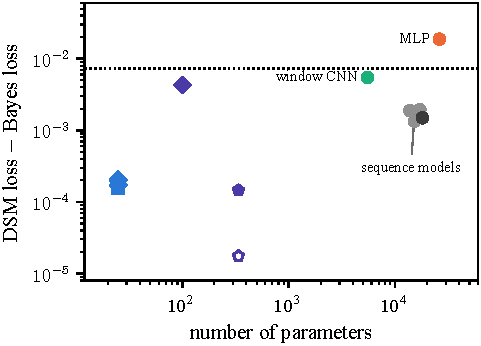
\includegraphics{fig_params}
  \caption{DSM loss above the Bayes loss against the number of parameters, Laplace chain, $n=2048$, medians over seeds.
  Square: the mixture; diamonds: four other shift families (25 parameters) and the log-linear kernel learned by EM;
  pentagons: the neural kernel by EM (filled) and by maximum likelihood on clean sequences (open); circles: six networks
  trained by DSM on the clean sequences. Dotted: the best linear denoiser.}
  \label{fig:params}
  % src: tools/paper_figs/figs_v5.py::fig_params_dsm (E89; n_params from E56 kernels.csv and E87 curves.csv)
\end{figure}

\begin{table}[!htbp]
  \caption{The six networks: the hyperparameters screened, the configuration kept, and its number of parameters. Every
  configuration kept predicts the noise.}
  \label{tab:networks}
  \centering
  \small
  \begin{tabular}{@{}llll r@{}}
    \toprule
    network & screened & kept & learning rate & parameters\\
    \midrule
    global MLP   & hidden $(128,128)$, $(256,256)$ & $(128,128)$ & $10^{-3}$ & 26{,}016\\
    window CNN   & radius $2,4,8$; width $64,128$ & radius 4, width 64 & $10^{-3}$ & 5{,}505\\
    TCN          & channels $32,64$; dilations $1,2,4,8$ & 32 channels & $10^{-3}$ & 17{,}057\\
    BiGRU        & hidden $32,64$ & 32 & $10^{-3}$ & 15{,}169\\
    transformer  & $(d,\text{heads},\text{layers})=(32,4,2),(64,4,2),(64,4,4)$ & $(32,4,2)$ & $3\times10^{-3}$ & 18{,}057\\
    U-Net        & channels $16,32$ & 16 & $10^{-3}$ & 13{,}713\\
    \bottomrule
  \end{tabular}
  % src: outputs/E03/params_confirm.json (grids), outputs/E03/winners.json, outputs/E03/confirm.csv (n_params)
\end{table}

\paragraph{Training.} Denoising score matching on the clean training sequences: each example gets a noise level drawn
from the twelve and fresh noise at every step; batch 64, Adam, gradient clipping at 1, 32{,}000 steps. For each
architecture, the grid of \cref{tab:networks}, two learning rates and two output parameterisations were screened on
four separate seeds, and the best configuration was kept for every $n$. Kernels and networks are tested on exactly the
same sequences.
% src: outputs/E03/params_confirm.json; tools/paper_figs/make_paper_figures.py::_paired_e03

\paragraph{Results.} \Cref{fig:networks} puts the six networks on one plot with the two kernels learned by EM. The
global MLP is the worst at every $n$, and the window CNN stops improving near the best linear denoiser. The four
sequence models keep improving with $n$, and the BiGRU is the best network at every $n$, still 3.5 to 11 times above
the neural kernel learned by EM (median per-seed ratios). The neural kernel is below each of the six networks in every
seed at every $n$.
% src: E89 per-seed ratios E87 / E56 energy: bigru 3.5, 4.2, 4.8, 11.2; tcn 4.4-14.2; unet 5.7-14.5; transformer
% 5.2-12.1 (8/8 every n)

\paragraph{Networks at their best.} The recipe above (constant learning rate, no weight averaging, 32{,}000 steps)
leaves the MLP and the window CNN on their last checkpoint at large $n$, so we retrained the networks under the recipe
of a diffusion U-Net: Adam with a linear warm-up over 1{,}000 steps, gradient clipping at 1, an exponential moving
average of the weights (decay 0.999), batch 128, $2^{17}$ steps, two learning rates ($10^{-3}$, $3\times10^{-4}$), with
wider variants (MLP with 512 units, window CNN with 256 channels and radius 8, TCN with 64 channels, BiGRU with 128
units), on 2{,}048 to 131{,}072 clean sequences, 4 seeds, the same test sequences. The best network is a BiGRU at every
$n$; its excess DSM loss is $4.3\times10^{-4}$ at $n=2048$ (three times below the standard recipe), $1.2\times10^{-4}$
at $32{,}768$ and $8.4\times10^{-5}$ at $131{,}072$. The window CNN improves with width and radius but stays above
$10^{-3}$. On the same seeds, the neural kernel learned by EM from 2{,}048 noisy sequences has $1.25\times10^{-4}$, the
mixture $1.05\times10^{-4}$, and the neural kernel fitted on 2{,}048 clean sequences $1.9\times10^{-5}$.
% src: E80 (frozen 20 Nov 2026), E89 medians over seeds 0-3; read_e80: P1-P4 and P6 confirmed, P5 falsified

\begin{figure}[!htbp]
  \centering
  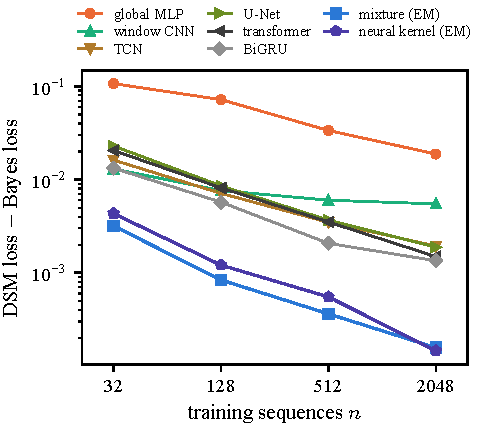
\includegraphics{fig_networks}
  \caption{The six networks against the mixture and the neural kernel learned by EM: DSM loss above the Bayes loss.
  Laplace chain, medians over seeds (8 for the networks, 16 for the kernels), same test sequences.}
  \label{fig:networks}
  % src: tools/paper_figs/figs_v5.py::fig_networks_dsm (E89: E87 networks, E02a rescored, E56)
\end{figure}


\section{Memorization}
\label{app:memorization}

\paragraph{Training and test losses.}

The DSM loss of \cref{eq:dsm} has a floor: on fresh data no denoiser beats the exact posterior mean, which BP
computes with the true kernel; we call its loss the Bayes loss. We retrain the six networks of \cref{tab:networks} on
the Laplace chain with the same data and recipe, 8 seeds, and record at twelve checkpoints between 250 and 32{,}000 steps
the DSM loss on the training sequences (one fixed noise draw per sequence and level) and on the 2{,}048 test sequences,
with the Bayes loss on the same draws. With 32 training sequences (\cref{fig:memorization}a) the training loss of five
networks falls far below the Bayes loss while their test loss rises, to two or three times the Bayes loss by 32{,}000
steps. The window CNN, the smallest and most local network, stays near the
Bayes loss on both. With 2{,}048 sequences (\cref{fig:memorization}b) training and test losses agree to within $0.01$.
\Cref{fig:memorization}c shows the test loss above the Bayes loss at each network's selected checkpoint, with BP on the
neural kernel fitted on clean sequences below every network in every seed.

\begin{figure*}[!htbp]
  \centering
  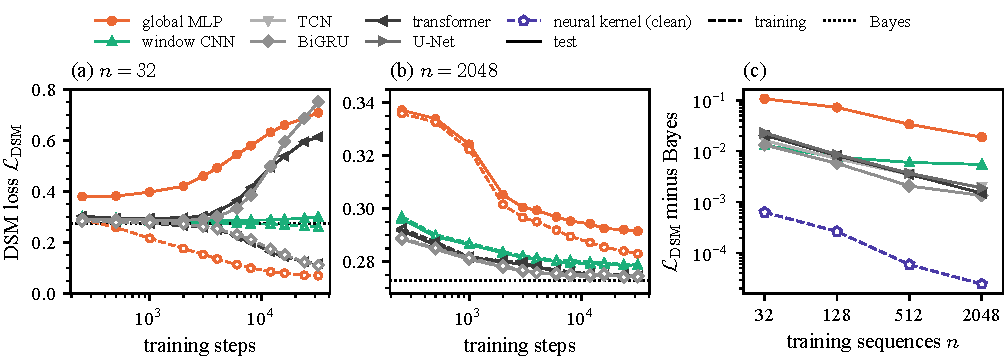
\includegraphics{fig_memorization}
  \caption{Memorization, Laplace chain. (a, b) Training (dashed, open markers) and test (solid) DSM loss of four of
  the networks along training, with $n=32$ and $n=2048$ training sequences. Dotted: the Bayes loss, BP with the true
  kernel. (c) Test DSM loss minus the Bayes loss on the same sequences, for each network at its selected checkpoint,
  against $n$; pentagons: BP with the neural kernel fitted on the clean sequences. Medians over 8 seeds.}
  \label{fig:memorization}
  % src: tools/paper_figs/figs_v4.py::fig_memorization on outputs/hpc_E87_s{0,4} (curves.csv, floors.csv), frozen
  % 19 Nov 2026; read_e87: G1 ok, P1-P4 confirmed
\end{figure*}

\paragraph{Do the samples copy the training sequences?}
\label{app:memorization-gen}
In the diffusion literature memorization means that generated samples reproduce training data
\cite{gu2023memorization}. We test it on the Laplace chain and on the Allen--Cahn field at $\Theta=0.3$, with
$n\in\{32,128,512,2048\}$ training sequences and 4 seeds. Every model generates 2{,}048 sequences with the same
ancestral sampler: 400 geometric steps from $t=3$ to $t=0.005$, the posterior mean as the last readout, and the same
sampler noise for every model. For a sample let $d_1\le d_2$ be its Euclidean distances to the two nearest training
sequences; it counts as a copy when $d_1/d_2<1/3$ \cite{gu2023memorization}. We also report the median of $d_1$
divided by the same median measured against $n$ new draws of the chain, which is 1 when the samples are no closer to
the training sequences than to unseen ones, and the sliced Wasserstein-2 distance to 2{,}048 new draws. The models are
BP with the kernels fitted on the same $n$ sequences, the neural kernel by EM from their noisy versions and by maximum
likelihood on the clean ones (and, on the chain, the $C=8$ mixture by EM), rebuilt from their stored parameters; and
five networks of \cref{tab:networks} (all but the TCN), retrained by DSM on the clean training sequences for
32{,}000 steps with noise levels drawn log-uniformly in $[0.005,3]$, read out at the checkpoint selected on validation
sequences and at the end of training. Two references bracket the scale: new draws of the chain, and the empirical
optimum, the exact minimizer of the DSM loss on the training set, $\mathbb E[\mathbf a\mid\mathbf x]=\sum_j
w_j\mathbf a_j$ with $w_j\propto\exp(-\|\mathbf x-e^{-t}\mathbf a_j\|^2/2\Delta_t)$, a perfect memorizer.

The empirical optimum copies every sample at every $n$ and new draws copy none, so the test detects copying
(\cref{fig:memorization-gen}). No kernel produces a copy, in any seed, at any $n$, on either data set, and the distance
ratio of every kernel stays between $0.99$ and $1.01$. Trained to the end on 32 sequences, the global MLP copies $45\%$
of its samples on the chain and $49\%$ on the field, the BiGRU $10\%$ and $12\%$, the transformer $5\%$ and $6\%$, the
U-Net about $1\%$ and the window CNN none; with 128 sequences at most $2.1\%$, and none from 512 on. At the selected
checkpoint no network copies, in any seed, at any $n$. Not copying is not the same as sampling well: with 32 and 128
sequences the selected global MLP stops so early that its samples are far from the chain (sliced $W_2$ near $5$,
against $0.04$ to $0.06$ for new draws), and at every $n$ the samples of every kernel are closer to the chain than those
of every network. The train--test gap of the DSM loss agrees: for the kernels it is at most $0.004$ at every $n$, the
order of the true kernel's own gap (up to $0.003$, the noise of a loss averaged over few sequences), against $0.04$ to
$0.65$ for the networks trained to the end on 32 sequences.
% src: tools/core/read_e92.py on outputs/hpc_E92_{laplace,field}/memorization.csv (E92, frozen 21 Nov 2026, amendment 1):
% G1 worst 2.0e-7, G2 worst 0.000; P1, P2, P4 confirmed; P3, P5 falsified. Seed means: frac_mem n=32 _final chain/field
% mlp 0.448/0.492, bigru 0.103/0.122, transformer 0.052/0.056, unet 0.009/0.013, window 0/0; n=128 max 0.021 (mlp
% field); med_ratio kernels 0.992-1.005; sw2 mlp_sel n=32/128 5.24/5.11 chain, 5.27/4.98 field, exact 0.043-0.058;
% DSM test-train kernels max 0.0043 (energy_em chain n=32), oracle max 0.0032; nets _final n=32 0.036-0.648.

\begin{figure*}[!htbp]
  \centering
  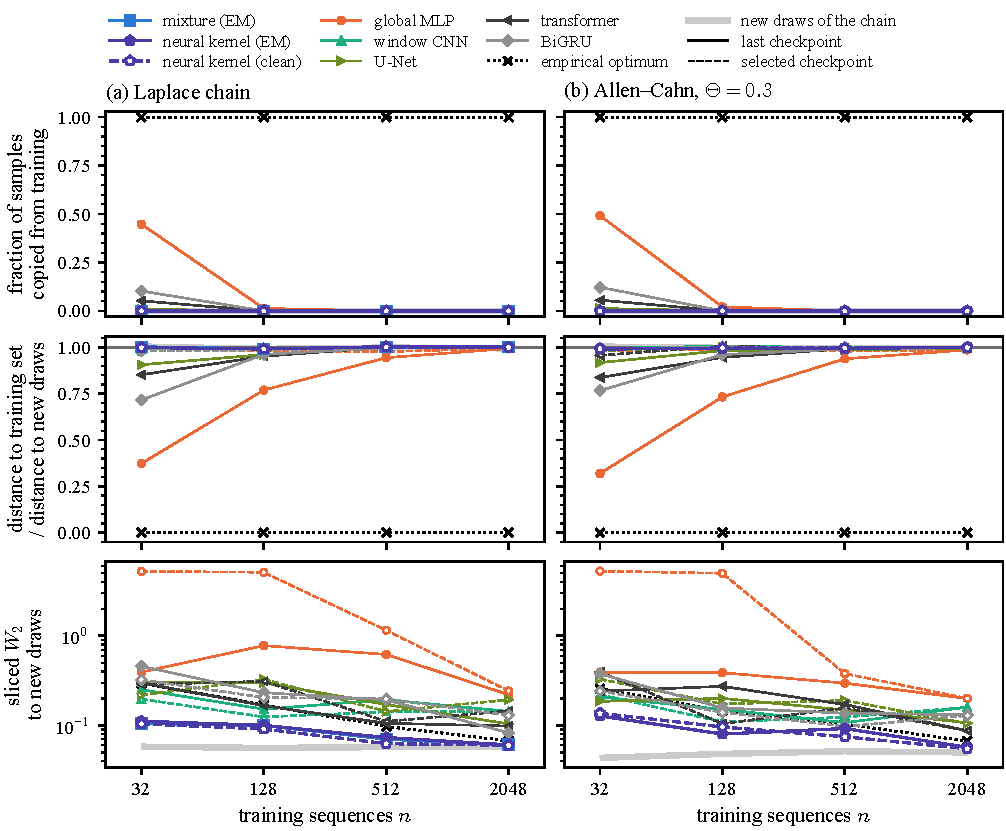
\includegraphics{fig_memorization_gen}
  \caption{Do the samples copy the training sequences? (a) Laplace chain, (b) Allen--Cahn field at $\Theta=0.3$,
  against the number $n$ of training sequences. Top: fraction of the 2{,}048 generated sequences that are copies,
  $d_1/d_2<1/3$. Middle: median distance to the nearest training sequence over the same median against $n$ new draws.
  Bottom: sliced Wasserstein-2 distance to new draws. Networks at the end of training (solid, filled markers) and at
  the selected checkpoint (dashed, open markers); thick grey: new draws of the chain; dotted crosses: the empirical
  optimum of the DSM loss. Means over 4 seeds.}
  \label{fig:memorization-gen}
  % src: tools/paper_figs/figs_v5.py::fig_memorization_gen on outputs/hpc_E92_{laplace,field} (E92, frozen 21 Nov 2026)
\end{figure*}

\section{Data that are not first-order Markov}
\label{app:nonmarkov}

\paragraph{Second-order chains.} $a_k=\phi_1a_{k-1}+\phi_2a_{k-2}+\varepsilon_k$ with Laplace noise,
$\phi_1=0.85(1-\phi_2)$ so that neighbouring sites keep correlation $0.85$, $\phi_2\in\{-0.3,0,0.1,0.2,0.3,0.4,0.6\}$,
$d=32$, $n\in\{128,512,2048\}$, 8 seeds, the networks and EM of the Laplace chain. The exact score is grid BP on pairs
with the true kernel. BP on pairs uses the state $(a_{k-1},a_k)$, a first-order chain, with a mixture kernel on the pair
learned by the same EM; the learned $\phi_2$ is within $0.01$ of the truth. BP plus a learned correction
(\cref{fig:nonmarkov}) feeds the posterior mean of first-order BP, with a kernel fitted on the clean sequences, to a
BiGRU of the recipe of \cref{app:networks}, which outputs a correction to the score and is trained on the DSM loss;
with the correction at zero it is BP, and its untrained output agrees with BP to $10^{-14}$. It is trained on 512 and
2{,}048 sequences, 4 seeds. On a hidden-regime chain, whose kernel switches between two laws, it is also below both BP
and the BiGRU.
% src: E62 (frozen 6 Nov 2026), E81 (frozen 20 Nov 2026; read_e81 G1 1.5e-14, P1-P5 confirmed), via E89

\paragraph{Fractional Gaussian noise.} fGn with Hurst index $H$ is the stationary Gaussian sequence with unit variance
and correlation $r(k)=\frac12\big(|k+1|^{2H}-2|k|^{2H}+|k-1|^{2H}\big)$ at lag $k$, first-order Markov only at
$H=\frac12$, where it is white noise. We use $H\in\{0.3,0.5,0.6,0.7,0.8,0.9\}$, $d=32$, $n=2048$, 8 seeds. The data are
Gaussian, so the exact score is linear, $\mathbf S_t(\mathbf x)=-(e^{-2t}\boldsymbol\Sigma+\Delta_t\mathbf I)^{-1}
\mathbf x$ with $\Sigma_{ij}=r(|i-j|)$, and so is the score of any Gaussian chain. The closest first-order chain matches
$r(1)$, the closest second-order chain $r(1)$ and $r(2)$; their scores give the two lines of
\cref{fig:nonmarkov-delta}b in closed form, and $\delta$, the Kullback--Leibler divergence per site from the data to the
closest first-order chain, is one between Gaussian laws. First-order EM--BP is within 1.4 to 6.8\% of the best
first-order chain at every $H\neq\frac12$: the kernel is learned as well as the model allows. The window CNN is below it
in every seed at $H=0.3$, $0.7$, $0.8$ and $0.9$, and in 5 of 8 at $H=0.6$, already at $\delta=2.6\times10^{-3}$ nats per
site. BP on pairs is below first-order BP in every seed at every $H\neq\frac12$, and below the CNN in every seed at
$H=0.6$ and $0.9$.

\paragraph{The distance to first-order Markov.} \Cref{fig:nonmarkov-delta}a puts the second-order chains and fGn on one
axis, $\delta$. On the second-order chains the advantage of the first-order kernel shrinks steadily as $\delta$ grows;
fGn falls off this curve, because its correlations extend over many lags, so that the best first-order chain is further
from the data, in denoising loss, than on a second-order chain at the same $\delta$. What sets the break-even point is
that loss, not $\delta$. Two other departures, a global latent variable and long-range couplings, were measured only in
the relative score error, with the same steady decline as on second-order chains.
% src: E83 (frozen 19 Nov 2026) via E89: first/floor1 1.014-1.068; window < first 8/8 at H=0.3,0.7,0.8,0.9, 5/8 at 0.6;
% pair < first 8/8 at H != 0.5; pair < window 8/8 at H = 0.6, 0.9 (4/8 at 0.7, 0.8; 0/8 at 0.3). Calibration delta from
% E62.json / E83.json. Thesis exp_21_clean for the global-latent and long-range families (relative error only).

\begin{figure*}[!htbp]
  \centering
  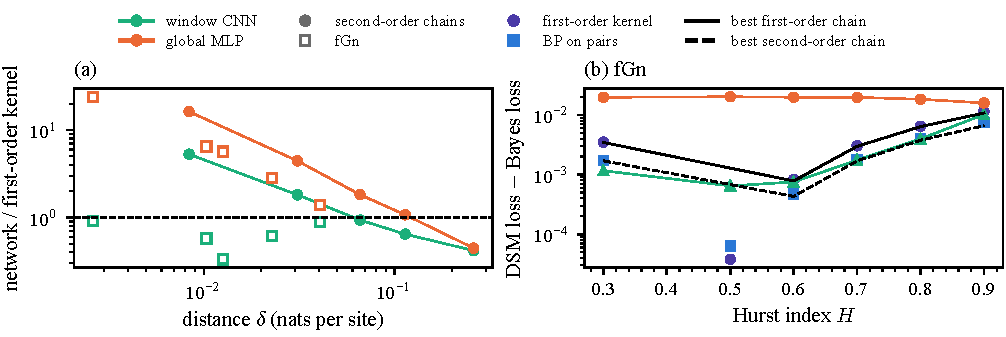
\includegraphics{fig_nonmarkov_delta}
  \caption{(a) Excess DSM loss of a network divided by that of first-order EM--BP, against the distance $\delta$ to the
  closest first-order chain: second-order chains (filled) and fGn (open), $n=2048$, medians over 8 seeds. Above the
  dashed line the kernel is more accurate. (b) fGn against $H$: excess DSM loss of the models, and of the best
  first-order (solid) and second-order (dashed) chains, in closed form.}
  \label{fig:nonmarkov-delta}
  % src: tools/paper_figs/figs_v5.py::fig_nonmarkov_delta_dsm (E89 on E62, E83; delta from the calibrations)
\end{figure*}

\section{A tree with hidden nodes}
\label{app:tree}

The tree has a root $a_0\sim\mathcal N(0,1)$ and every child is $0.85$ times its parent plus Laplace noise of variance
$1-0.85^2$, the kernel of the Laplace chain; at depth five its 32 leaves, read left to right, are the observed sequence,
and two leaves whose lowest common ancestor is $h$ levels up have correlation $0.85^{2h}$. BP on the tree has upward and
downward messages on the same 401-point grid and is exact; it gives the score of the noisy leaves and the pair posterior
of every link, so EM works as on the chain, from one noisy view of the leaves of each tree. We learn the mixture and
the neural kernel this way, and compare with the paper's method applied blindly, a first-order chain kernel on the
leaves, and with the six networks trained by DSM on the clean leaves, $n\in\{128,512,2048\}$, 8 seeds. At $n=2048$ the
neural kernel's excess DSM loss is $1.0\times10^{-4}$ and the mixture's $1.4\times10^{-4}$, against $4.5\times10^{-3}$
for the best network, a BiGRU; the chain kernel, with the wrong graph, stays at $2.3\times10^{-2}$, above every
network. On this tree the best linear denoiser, $3.8\times10^{-3}$, is itself below every network.
% src: E82 (frozen 20 Nov 2026; read_e82 G1-G3 pass, P1-P5 confirmed) via E89 medians.

\section{The Allen--Cahn field}
\label{app:field}

\paragraph{What the field looks like.} \Cref{fig:field} shows the chain of \cref{sec:allen-cahn}. The potential has two
wells at $\phi=\pm1$ (a). At $\Theta=0.3$ a sample sits in one well or the other and jumps between them; at $\Theta=2$
the heat dominates and the field looks like a Gaussian chain (b). The one-site law at low and high temperature (c). The exact kernel at $\Theta=0.3$ changes shape with the current value
$a$: broad between the wells, skewed towards the well from $a=0.6$, narrow and one-sided inside it (d). A shift family
can move the centre of $K(a'\mid a)$ with $a$, but not its shape. We work with the standardised field $a=\phi/s$, which
has unit variance, and choose the lattice spacing so that neighbouring sites have correlation $0.85$ at each
temperature.
% src: outputs/E32/cells.json (h = 1, 0.419, 0.226, 0.150 at Theta = 0.3, 0.5, 1, 2; rho1 0.848-0.850)

\begin{figure*}[!htbp]
  \centering
  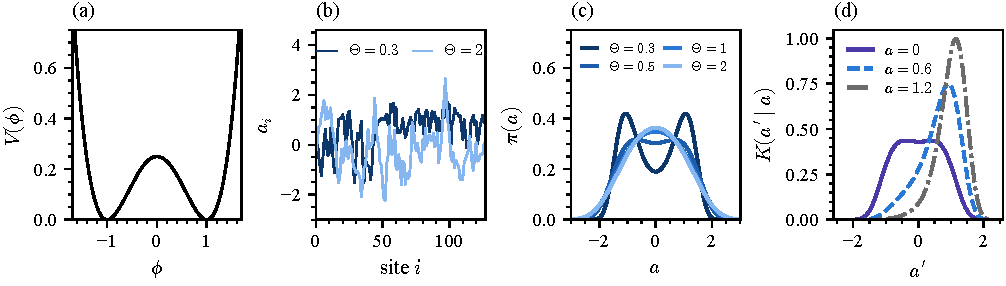
\includegraphics{fig_field}
  \caption{The Allen--Cahn field. (a) The double-well potential $V(\phi)$. (b) One exact sample of the standardised
  field at $\Theta=0.3$ and one at $\Theta=2$. (c) Law of one site at the four temperatures. (d) The exact kernel
  $K(a'\mid a)$ at $\Theta=0.3$ for three current values $a$.}
  \label{fig:field}
  % src: closed form and exact sampling (E32 cells), tools/paper_figs/figs_v2.py::fig_field
\end{figure*}

\paragraph{More kernels.} All are learned by EM through BP from noisy sequences. The \emph{site energy} (5 parameters)
has the form of the lattice energy, $K(a'\mid a)\propto\exp(-(a'-a)^2/2\gamma-f(a)-f(a'))$ with $f$ a polynomial of
degree four. The \emph{tilted spline} (25) is a random walk tilted by a learned function of $a'$. The \emph{free mixture}
(24) is a mixture of four Gaussians for the pair $(a,a')$, read as a conditional law. The \emph{log-linear} kernel
(100) and a \emph{mixture density network} (1{,}516) know nothing about the field. The neural kernel (337 to 1{,}185
parameters) and the shift mixture (25) are those of \cref{sec:kernel-families}. The networks of \cref{tab:field} are a
window CNN and a transformer, each trained in two ways on the same noisy sequences as EM, and we report the best of the
four; the U-Net is a diffusion U-Net with $1.2\times10^7$ parameters, trained on the clean sequences.

\paragraph{Results.} \Cref{tab:field} gives the errors relative to the best linear denoiser. Every kernel whose shape can
change with $a$ beats the best of the four networks at every temperature, including the ones that know nothing about
the field. The shift mixture is no better than the linear denoiser at any temperature. The site energy, which has the
right form, is the most accurate model everywhere. The U-Net is a much stronger network than the other four, and the
neural kernel still beats it in 30 of 32 paired seeds with 2{,}048 sequences; the U-Net needs 8{,}192 sequences to
reach the neural kernel's error.
% src: figures/tab_field.tex (tools/paper_figs/make_paper_figures.py::tab_field); E55 finished cells: wins 8/8/8/6;
% U-Net at N=8192 reaches the kernel's N=2048 error in every cell

\begin{table}[!htbp]
  \caption{Allen--Cahn field: relative score error divided by that of the best linear denoiser, from 2{,}048 training
  sequences; mean over 16 seeds (8 for the neural kernel and the U-Net). Best of four: a window CNN and a transformer,
  each trained in two ways on the same noisy sequences as EM. Dashes: not run.}
  \label{tab:field}
  \centering
  \small
  \setlength{\tabcolsep}{3.5pt}
  \begin{tabular}{@{}lrcccc@{}}
\toprule
 & param. & $\Theta=0.3$ & $0.5$ & $1$ & $2$\\
\midrule
site energy & 5 & 0.033 & 0.072 & 0.141 & 0.169\\
neural kernel & 337--1{,}185 & 0.122 & 0.218 & 0.368 & 0.664\\
free mixture & 24 & 0.140 & 0.292 & 0.373 & 0.459\\
tilted spline & 25 & 0.060 & 0.134 & 0.280 & 0.428\\
log-linear 2-D & 100 & 0.184 & -- & 0.428 & --\\
MDN & 1{,}516 & 0.228 & 0.422 & 0.738 & 0.838\\
shift mixture & 25 & 1.004 & 1.004 & 1.014 & 1.021\\
\midrule
U-Net & $1.2\times10^{7}$ & 0.215 & 0.399 & 0.692 & 0.951\\
best of four &  & 0.484 & 1.174 & 2.157 & 3.044\\
\bottomrule
\end{tabular}

  % src: figures/tab_field.tex = tools/paper_figs/make_paper_figures.py::tab_field (E33, E43, E60, E55 finished cells)
\end{table}

\end{document}
